% Chapter 1

\chapter{Deep Polarization-Based Monocular Depth Estimation} % Main chapter title

\label{Chapter5} % For referencing the chapter elsewhere, use \ref{Chapter1} 

%----------------------------------------------------------------------------------------

% Define some commands to keep the formatting separated from the content 


%----------------------------------------------------------------------------------------

This chapter is dedicated to depth estimation using a polarimetric monocular. We seek to infer, from a unique polarimetric view, a dense depth map while eliminating the recurrent problems of standard methods (saturation, specularity/reflection implied erroneous estimation, etc.). Indeed, since data from uncontrolled outdoor environments can be subject to numerous alterations, whether meteorological or due to the sensor, the algorithm should be robust and take into account all these characteristics. To this end, we propose a polarization-based approach of monodepth (MD).\\

As detailed in Chapter \ref{Chapter2}, a remarkably large number of approaches have been used to infer a depth map from a single view. Due to the need for data representativeness, a vast majority of approaches rely on colorimetric images. On the contrary, it is noteworthy that all these methods show increased capabilities and allow consistent estimation. Consequently, MD represents a promising candidate and above all a significant baseline for altered data assessment. Among the numerous works in literature, it is possible to extract a method that has — in part — catalyzed the craze for MD, Godard et al.\cite{godard2017unsupervised}. 
This approach is very promising since it uses two processes exportable to polarimetry: unsupervised learning and generically formulated loss through the statement of perspective geometry. For the sake of robustness, the unsupervised approach is preferred since it negates the cost of data annotation. Indeed, ground truth depth maps are tedious to acquire and often very inaccurate. As a result, the non necessity of them reduces the complexity of training but at the cost of a loss function of a different formulation. 
Secondly, the cost function shows adaptation and generalization capabilities. Borrowing the formulation of perspective geometry, it is therefore functional in all image spaces. It allows reconstructing a depth map from two views during training similarly to stereovision reconstruction algorithms.
By all these aspects, \cite{godard2017unsupervised} is a process exploitable with polarization since the prerequisites are not in conflict with space. 
In a second step, Godard et al. improved their method to include aspects of multi-scale, masking of immobile/occlusion zones. In \cite{godard2019digging}, a field of possibilities is then opened, showing it is possible to limit the cost function and thus to add additional discriminant criteria to it.
From this last contribution, we propose Polarimetry to Depth (P2D), a method adapted to polarimetric imaging. By extending the loss function to include a polarimetric term we propose a new network that will be subject to the constraints of perspective geometry — which are valid for any image pair — as well as sensitive to polarization data. Due to the prerequisites of such approaches, we propose a brand new data set that will be representative of road scenes. Plus, since one of the core objectives is to be invariant to weather changes, we have aggregated this set of images captured in diverse conditions. The proposed approach has been validated by the various experiments made possible by this dataset.
Ultimately, since P2D showed some flaws in some experiments, we proposed other fusion-based methods. 
Indeed, P2D seems to be too relying on visual features, and thus showing weaknesses of genericity, we concluded it was necessary to use both polarimetric and colorimetric information. To accomplish this task and thus to group two very different types of images, we had to reverse-engineer multiple fusion methods and evaluate their validity in relation to the context. Ultimately, we propose a cascaded network method as well as a cascaded double loss to finally discriminate only the normals without passing specifically in the 3D space. With this approach we reduce the impact of inaccuracies when changing consecutive spaces and therefore address the problem in a more appropriate way.

\section{Introduction}
The scene reconstruction represent a major task in computer vision. It offers an observation of the three-dimensional world accurate in shape, size and geometric structure. This explains its great usefulness since it allows an increased understanding and thus a massive potential of application.

There are multiple possibilities to obtain a three dimensional scene reconstruction. Each method has its own constraints. A pair of cameras will subsequently allow the reconstruction by stereovision and operating a registration and a camera-to-camera projection.
A mobile 2D camera, on the other hand, will allow the reconstruction of the scene using registration through a sequence of images using Visual Odometry.
In each of these cases, the methods suffer from the dynamicity of the scenes and therefore produce artifacts. To be specific, the monocular method operating a visual odometry-based registration is valid only for static parts of the scenes.

To eliminate these drawbacks, some methods are DL-based and show improved capabilities but especially a lifting of past constraints.Monocular supervised methods learn the direct correspondence between an input image and a ground truth image. These preliminary methods although reducing the constraints requires a large dataset of images and, above all, their corresponding accurate reconstruction which makes them difficult to use, especially with a new data type. 

To avoid aggregating heavy and imprecise datasets, unsupervised methods do not need ground truth at the cost of a more complete loss function. Indeed, a simple observation is databases are quite unreliable. Specifically, when it is necessary to have an accurate depth map, the acquisition processes are unaccurate enough. Essentially, for this kind of acquisition, a LiDaR is used. As follows, it will project a laser band and measure the return time of the reflected beam. This is valid on one condition, that the laser is undiverted and therefore returns, unaltered, to the sensor. Under ideal conditions this method is extremely efficient. On the other hand, a substantial majority of approaches address the problem of reconstruction in urban scenes. One observation is that cars are reflective and therefore subject to laser deflection. Also, in uncontrolled areas like these, there may be multiple surfaces modifying the light rays (windows, mirrors, ...). Ultimately, outdoor acquisitions are subject to climate change, rain, and therefore water accumulation on the tracks/objects which modify the interaction of light with the surfaces. It is then possible to see the datasets are acquired only under certain conditions and that they periodically produce artifacts/imprecisions.
As a reminder, a DCNN is generic at most as much as the dataset on which it has learned. Thus, from these observations, despite a non-supervised approach and consequently a loss supposed to bring this genericity, the approaches suffer from various weaknesses. Specifically, the estimation of specular surfaces is often incorrect and due to the nature of the operating scenes, these algorithms seem difficult to deploy in real conditions of use (for autonomous cars for example).

We propose using the luminous charateristics as an attachment point for our method. While previous approaches suffered from their lack of understanding of certain light phenomena we propose to use them to the advantage of our method. While specularity was mostly neglected and poorly estimated in the color space, it is particularly clearly defined in the polarimetric space. As follows, we aim at keeping the accurate estimates of the previous algorithms while aggregating the knowledge of surface-to-light interraction. Given a sufficient number of representative polarimetric images, we aim to produce high quality accurate reconstructions by exploiting both visual features and polarization data.
A DL network will then be fed with polarimetric images and constrained by a particular loss integrating polarization specific terms. In a first step, we propose a method that is only dependent on polarimetric images. In a second step, we propose to investigate fusion methods that keep the viability of past methods while adding extra precision on specular areas. 


\section{Depth-to-polarization interconnections}

Since the core idea is to keep the unsupervised aspect to the learning, a link between the input image (polarimetric) and the desired output image (depth) is needed. In the case of colorimetry, the algorithms rely on the perspective geometry formulation. In other words, the approaches require visual features. 
It is possible to use this space in the colorimetric space but it will be restricted due to the absence of color. On the positive side, there is a direct link between the acquisition of the sensor and the depth, this thanks to the specularity.

\subsection{Normals to angle of polarization}

As detailed in Section \ref{Polar_explain}, polarimetric acquisition is very versatile and allows deducing many characteristic images. One of the strengths of this modality is that we have a direct measurement of the polarization angle. This angle can be very discriminating as shown in Chapter \ref{Chapter4}, but it could also be very useful for linking the modality to a depth map. \\
As a reminder, the polarization angle $\alpha$ is calculated as follows:

\begin{equation}
	\alpha = \frac{1}{2}\arctantwo(s_1, s_2).
\end{equation}


As  shown in  Figure  \ref{fig:found},  it  is  equally  possible  to  geometrically  represent this component of polarimetric information mixing peculiar and  perspective  geometry.

\begin{figure}[h]
	\centering
	\vspace{0.1cm}
	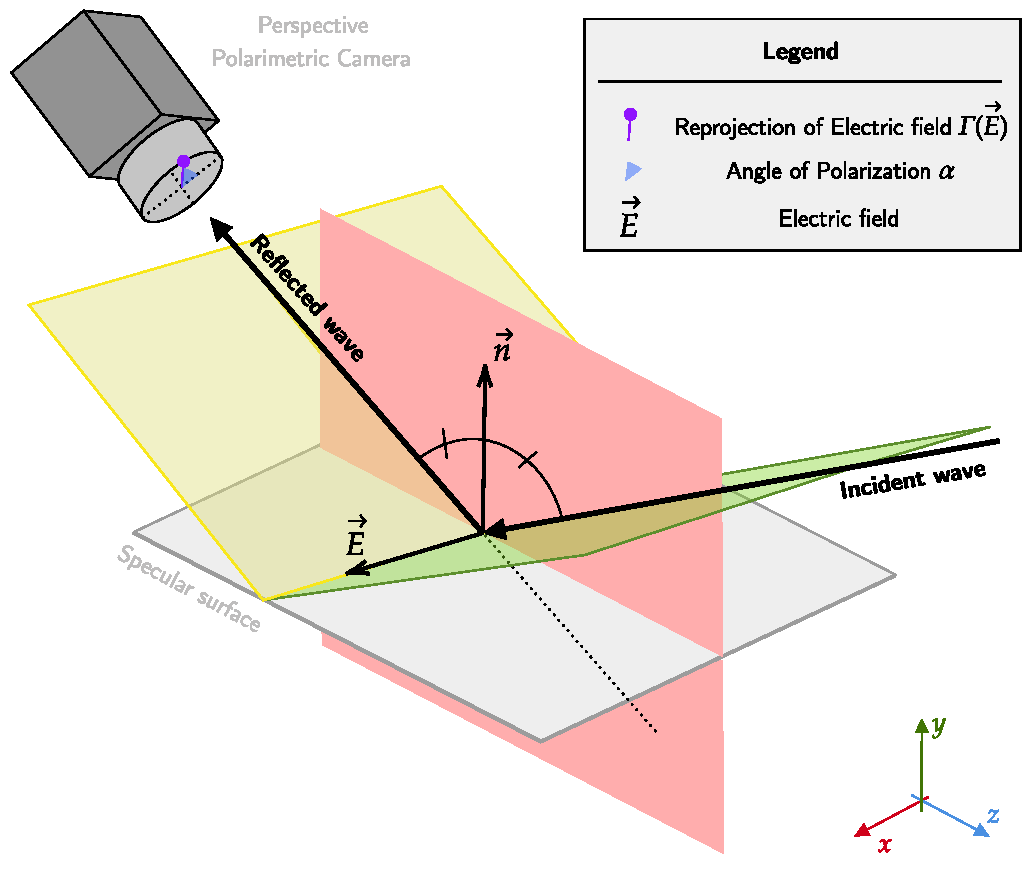
\includegraphics[keepaspectratio,width=.8\linewidth]{Figures/ECCV/foundations_prev.pdf}
	\caption{Illustration of imbrication of polarimetry peculiar and perspective geometry. Visual representation of angle of polarization measurement.}
	\label{fig:found}
\end{figure}

There is a definite relationship between $\alpha$ acquired and the plane normal. Provided that the surface is specular and reflects light, then a relation exists between the reference and the direction of the electric field $\vec{E}$ projection.
From this follows the possibility of deducing the normal $\vec{n}$ to the specular surface (i.e. a high degree of polarization $\rho$) since $\vec{E}$ is perpendicular to it. This statement is valid if and only if the surface is specular, which ensures perpendicularity between the two directions mentioned above. Otherwise, there would be no definite angle between $\vec{E}$ and $\vec{n}$ and therefore the equation would be neither differentiable nor -factually- optimizable. 
In order to guarantee the validity of the formulation, it is then necessary to discriminate using $\rho$ as a criterion since this acquired sensor parameter allows a quasi equivalence to the specularity measurement. 

\section{Towards a unified polarization-based method for depth estimation}
To infer a depth map from a single polarimetric image, we formulate a loss function supported by polarimetry-to-depth links. The accurate reconstruction is obtained by optimizing this function by a deep learning network in an unsupervised manner.
\subsection{Defining the loss}

Since the problem is unsupervised, the problem is not just to have the data and formulate a statistical function. Since we are not relying on ground truths, it is imperative to formulate an optimizable representative function that will take into account the polarimetric information. With the ambition of faithfully reconstructing the often neglected specular areas, we propose to build on similar work on reconstruction using polarization.

\subsubsection{Prior polarimetric reconstruction error}

The paper by Berger et al. \cite{berger2017depth} proposes an approach to minimize an error specific to polarimetric induced geometry. Drawing on the terms provided by Woodford et al. \cite{Woodford2008GlobalPriors}, the method consists in including a minimizable expression compelling a normal/polarization angle consistency.
It is consequently shown that constraining a cost function involving a polarimetry-specific geometry is valid. Furthermore, this minimization approach is operable when optimizing a deep learning model since it depends on both the input and output of the processing pipeline and therefore could guarantees a self-supervision capability. Nevertheless, the acquisition setup as well as the problem formulation highly influence the error calculation. Indeed, \cite{berger2017depth} proposed an azimuth to acquired angle of polarization comparison. This approach is consistent under peculiar conditions implying restricted calibration of the camera or azimuth to angle of polarization specific link hypothesis. For this reason, our method proposes an alternative but similar approach allowing standard calibration and a generalized loss term releasing the constraints and allowing for easier use in real word applications.


\subsubsection{Constraining the loss}

Fundamentally, the function to minimize includes a reprojection error term and a smoothing term. Our method P2D employs the photometric error proposed in~\cite{godard2019digging} since it has demonstrated its optimization and efficient convergence capabilities via deep learning. As a replacement for the edge aware first order smoothness, the second order derivative enhancement proposed by \cite{Woodford2008GlobalPriors} is used to encourage fine transitions counterbalancing the discontinuities induced by the polarization parameters.\\ 
First, one penalizes the photometric reprojection error:

\begin{equation}
L_r = \min_{t^\prime} \: pe(I_t, I_{t^\prime \rightarrow t}),
\end{equation}
with $t^\prime \rightarrow t$ the pose transformation between two consecutive views and $pe$ the reconstruction error:

\begin{equation}
pe(I_a, I_b) = \frac{\beta}{2} (1- SSIM(I_a, I_b)) + (1-\beta) ||I_a - I_b||_1.
\end{equation}


To comply with the specifications of a minimizable function, the reprojection error comprises the weighted combination of structural dissimilarity (DSSIM) and L1 difference penalizing the deviation per pixel of the reprojection. As described in the original paper, $\beta = 0.85$ is used.


In a second step, a smoothing term is used to encourage a precise estimation of the planes while taking into account the edges:

\begin{equation}
L_s = |\delta^2_xd_t^*| e^{-|\delta^2_x I_t|} + |\delta^2_yd_t^*| e^{-|\delta^2_y I_t|},
\end{equation}
where $d_t^* = d_t / \bar{d_t}$ is the mean-normalized inverse depth enforcing the depth to be dense while reconstructing the planes~\cite{wang2018learning} and the $\delta^2$ operator is defined according to the second order prior smoothness term $\mathcal{S}(\{j,k,l\})$ \cite{Woodford2008GlobalPriors}:
\begin{equation}
\mathcal{S}(\{j,k,l\},d_t^*)_x = \delta^2_x d_t^* = d_t^*(j) - 2* d_t^*(k) + d_t^*(l),
\end{equation}
with $\{j, k, l\}$ three neighboring pixels in the horizontal or vertical direction following the $x$-axis or $y$-axis orientation of the smoothing.

The weighted combination $L_{\textrm{diff}}$ of these two terms then allows for a precise reconstruction of the non-reflective (diffuse) areas.


\begin{equation}
L_{\textrm{diff}} = \mu L_r + \lambda L_s,
\end{equation}
with $\lambda$ a scaling parameter set to $1e^{-3}$ and $\mu$ a binary mask defined in \cite{godard2019digging} taking occlusion and displacement of pixels along sequences into account.

Now, by drawing inspiration from and generalizing the contribution in \cite{berger2017depth}, it is possible to include a third term into this loss to penalize poor reconstruction of reflective areas. By definition, polarization is defined by the orientation of the electric field. Consequently, it is possible to estimate the electric field as a function of a normal derived from a plane.

\begin{figure}[]
	\centering
	\vspace{0.2cm}
	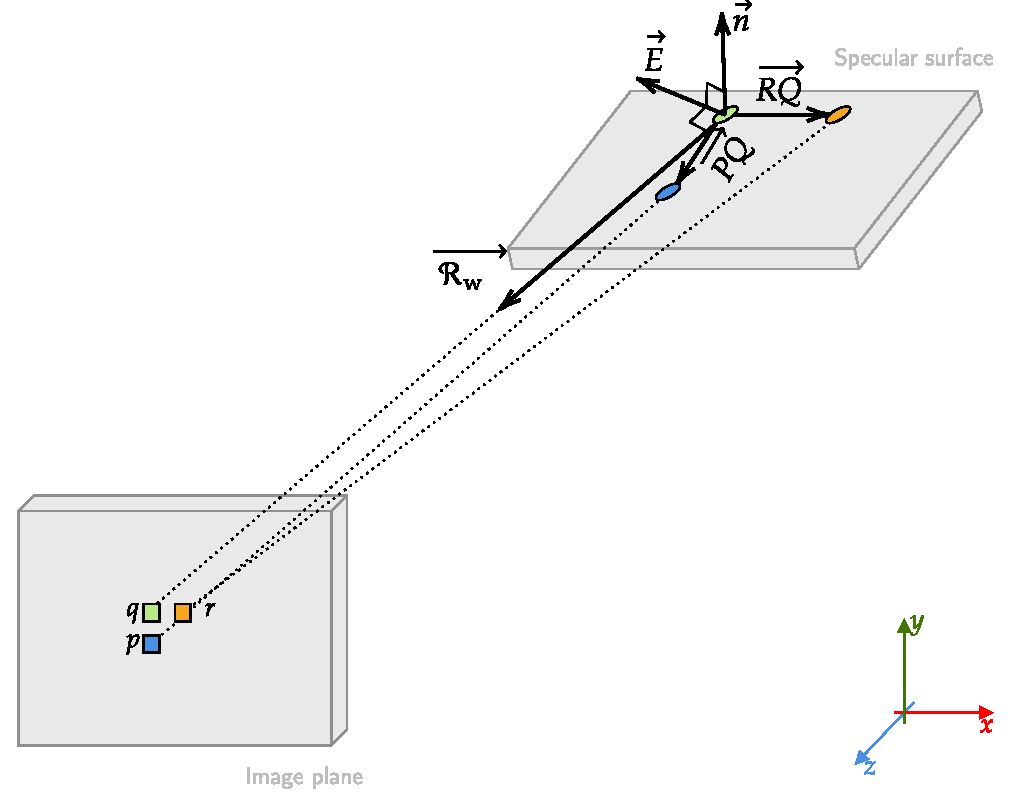
\includegraphics[keepaspectratio,width=.8\linewidth]{Figures/ECCV/foundation}
	\caption{Illustration of the electric field estimation method.}
	\label{fig:efromp}
\end{figure}

Let us consider three neighboring pixels $\{p, q, r\}$ in the layout presented in the Figure~\ref{fig:efromp}. This arrangement is organized such that it removes fronto-parallel planes related uncertainties. Then, the projection of these three adjacent pixels into 3D results in three points of a plane, respectively $\{ P, Q, R \}$. 
The local normal $\overrightarrow{n}$ is obtained via the cross-product of the two vectors $\overrightarrow{PQ}$ and $\overrightarrow{RQ}$ linking the points $\{P,Q,R\}$. By definition, the electric field $\overrightarrow{E(Q)}$ is perpendicular to the plane defined by the the normal and the reflected wave when considering specular surfaces. Following the definition, $\overrightarrow{E(Q)}$ at 3D point $Q$ can be deduced from the cross product between the local normal and $\overrightarrow{\mathcal{R}_\mathrm{w}}$ at the point $Q$ as follows:

\begin{equation}
\begin{split}
\overrightarrow{E(Q)} = &\Bigl[ \Big(\Pi(p,D(p)) - \Pi(q, D(q))\Big) \times\\& \Big(\Pi(r,D(r)) - \Pi(q, D(q))\Big) \Bigr]
\times \overrightarrow{\mathcal{R}_\mathrm{w}} ,
\end{split}
\end{equation}

where $\Pi(x,D(x))$ is the 3D projection of pixel $x$ relative to the disparity $D(x)$. In an optimal context, the polarization angle and the electric field maintain the same orientation and by extension the same angle relative to the reference as shown in the Figure~\ref{fig:cpol}. Conversely, when a depth map is incorrectly estimated, then the estimated local normal is inconsistent and consequently is the deduced polarization angle. Accordingly, we can add a term $C_{\textrm{pol}}$ to the loss penalizing the deviation of the normal.



As shown in equation \ref{backpro} and in Figure~\ref{fig:cpol}, to evaluate the deviation, it is necessary to back project the direction of the electric field onto the image plane and compare it with the angle of polarization $\alpha$:

\begin{equation}\label{backpro}
C_{\textrm{pol}}(q) = \rho(q) ~ \Big|\tan\big[\tan^{-1}\Big(\Gamma(\overrightarrow{E(Q)})\Big) - \alpha(q)\big]\Big| ,
\end{equation}
where $\Gamma$ is the back projection operator onto the image plane. 
Moreover, $\rho$ allows the scaling of the loss reinforcing the necessity for correlation between $\alpha$ and $\rho$.\\
\begin{figure}[]
	\centering
	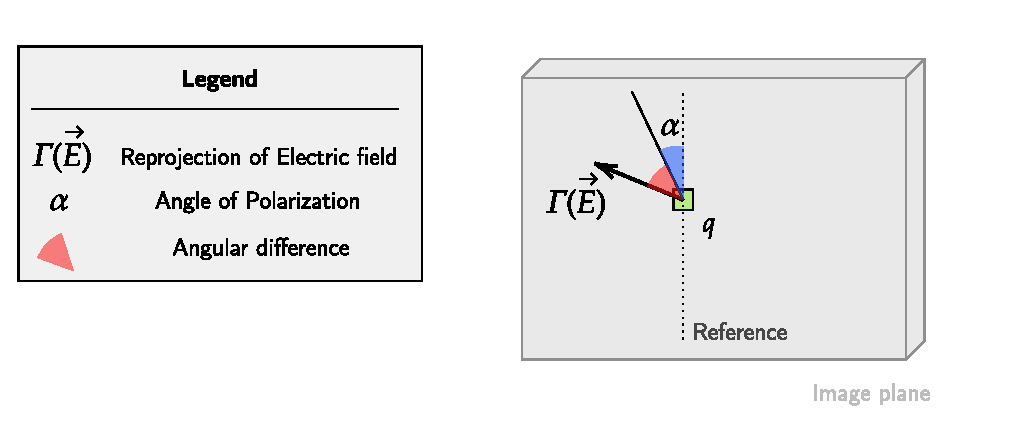
\includegraphics[keepaspectratio,width=\linewidth]{Figures/ECCV/Cpol}
	\caption{Angular difference visual representation. Here, the reference of the angle of polarization is vertical.}
	\label{fig:cpol}
\end{figure}


Since an angular differences is considered, and because this term will be combined with the reprojection term, the definition domains must be taken into account. The reprojection term clearly belongs to $[0,\infty[$ interval. To constrain the polarization term to the same interval, the absolute tangent is employed.
As a result, the polarimetric loss term becomes:
\begin{equation}\label{LPol}
L_{\textrm{pol}} = \frac{1}{N}\sum_{x \in \chi} C_{\textrm{pol}}(x),
\end{equation}
with $N$ the number of pixels $x$ in the set of reference image pixels $\chi$. Finally, the loss used to train the network is defined by: 

\begin{equation}
\Lambda =  L_{\textrm{diff}} + ~\tau ~L_{\textrm{pol}},
\end{equation}
\noindent
where $\tau$ is a binary mask derived from $\rho$ such that:
\begin{equation}
\tau(x) = \begin{cases} 1, & \mbox{ if } \rho(x) ~ \geq ~ 0.4\\
0, & \mbox{ otherwise}\end{cases}.
\end{equation}
The polarimetric term $L_{\textrm{pol}}$ is taken into account only if the degree of polarization is relevant. Since, the relevance of both $\rho$ and $\alpha$ are correlated, this mask ensure for a legitimate electric field estimation.
The final loss $\Lambda$ is then just composed of reprojection error when the image area is unpolarized. Polarization components, when consistent, are taken into consideration and penalize the inaccurate reconstruction of specular surfaces.

\subsection{Network architecture}

Following \cite{godard2019digging}, the network has an encoder-decoder architecture (a UNet with a ResNet 50 layout as shown in the Figure~\ref{fig:net}). It takes as input three-channel images obtained by concatenation of the intensity $\iota$, the polarization angle $\alpha$ and the degree of polarization $\rho$.
To overcome some inconsistencies related to the polarimetric modality and to consider exclusively areas with a minimum partial specularity, all values of lower than
0.4 are eliminated. This is justified by the fact that diffuse surfaces corresponding to low degree of polarization lead to a difference of $\pi/2$ between $\alpha$ and the electric field $E$.
When the disparity induced by the reprojection error is calculated, despite the accuracy of this calculation, the angular error will then tend towards $\pi/2$ leading the $L_{\textrm{pol}}$ function to tend towards infinity and thus causing exploding gradient problems.\\
Similarly, a perfect $\rho$ is physically unobservable which justifies an upper threshold. To combine a scale-factor effect and a regularization relative to physical property, the values are clipped to a maximum of 0.8.

\begin{figure}[t]
	\centering
	\vspace{.1cm}
	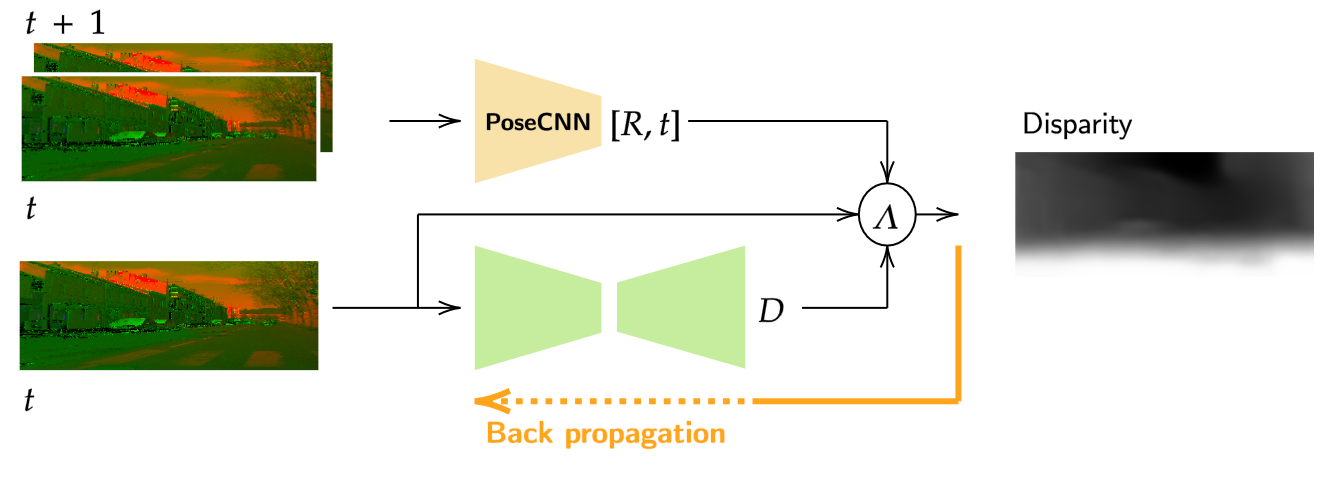
\includegraphics[keepaspectratio,width=\linewidth]{Figures/ECCV/diagramnet}
	\caption{Illustration of the network as well as the loss calculation strategy and its back propagation. Drawing inspiration from \cite{godard2019digging}, the depth estimation network is a UNet with a ResNet50 layout.}
	\label{fig:net}
\end{figure}

\subsection{Experiments}

\subsubsection{Implementation details}

\indent
\textbf{Datasets.} The training dataset was acquired during both dry and rainy weather such that the experiments would highlight the capacity of polarimetric modality in diverse conditions.
All acquisitions were made with an affordable polarimetric camera, the Basler Ace aca2440-75um POL, consisting of a Sony IMX250MZR sensor delivering a resolution of 2448~x~2048 pixels.
The camera was mounted on board a driving car, recording a total of approximately 7,000 images per weather condition. The final training dataset is composed of 13,400 images.
As for the evaluation dataset, it is composed of a completely independent set of 25 images, acquired separately from another view under mixed meteorological conditions.\\

\textbf{Ground truth. }Ground truth generation represents a critical point when it comes to addressing urban reconstruction problems.  Because of specularity, accurate depth evaluation is difficult since ground truth generation commonly rely on LiDAR sensors which are occasionally unreliable for measuring specular surfaces geometry due to reflection or transparency. Indeed, it would be a prerequisite to spray matte coating over all the specular surfaces of a complex urban scene wich is obviously unfeasible.
To overcome such difficulties, the reference disparity has been pre-calculated using SGBM \cite{hirschmuller2007stereo} and then refined by hand. It would have been possible to calculate the ground truth using a learning-based method. It should be considered the approach presented here is to improve deep learning methods since they typically fail on specular surfaces. Moreover, it is notable the vast majority of networks are trained on the same database which consists of images in favorable weather conditions. For these reasons, the choice of a refined SGBM eliminates learning biases while providing ground truth taking into account specular surfaces. This approach is unconventional but permits to conceive a global idea of the reliability of the results while allowing the computation of metrics. In addition, the disparity remains a relative value and therefore the impact of manual refinement is minor.\\


\textbf{Network training. }The network was trained on a machine consisting of a Nvidia Titan Xp (12GB memory) GPU, 128GB of RAM and two CPUs accumulating a total of 24 physical cores. 
We use the following parameters for all the networks: a batch size of 12, a learning rate of 1e-3 and a maximum of 30 epochs.
For a fast training, the images were downsampled without any interpolation method to maintain the physical properties. 
Following this routine, training with polarimetric images takes approximately 17 hours compared to 12 hours when training with intensity images only. 
The forward pass inference time is around 0.45 second per image in pure CPU processing.\\


\textbf{Hyper-parameters. } To define the set of hyper-parameters we conducted experiments to evaluate the final performance of each network. Table \ref{tab:hyper} shows the study conducted to define whether pre-training was necessary and which empyric parameters were suitable.\\


\textbf{Evaluation.} We compared the results of our method P2D with the competitive state-of-the-art method described in \cite{godard2019digging}. Our P2D receives as input the polarization parameters by concatenation of the three channels $\{\iota, \alpha, \rho\}$. For the method in \cite{godard2019digging}, we evaluate two versions. One version, $G_{\textrm{RGB}}$, using only intensity images and trained with the weights provided by the authors without fine-tuning. And, another version, $G_{\textrm{I}}$, trained in an end-to-end manner so that the network parameters are adapted to the intensity images at hand.\\


\textbf{Metrics. }The calculated metrics shown in the table \ref{resmet} represents popular assessments within the reconstruction community that have been proposed by Eigen et al. \cite{eigen2014depth}. They provide an unbiased and comprehensive measure of results. In particular, the $\delta$ values are calculated on the prediction/ground truth ratio and highlight an intrinsic precision of the reconstruction.\\

At last, the sky reconstruction accuracy $R_s$ is calculated as follows:
\begin{equation}\label{reconSky}
R_s = 1 - \Big(\frac{\hat{y}_s}{y_s}\Big),
\end{equation}
where $y_s$ is the sum of the binary masked pixels considered as sky in the ground truth and $\hat{y}_s$ the corresponding area in the prediction. This calculation is performed on the disparity, and one order of magnitude error deviation is considered acceptable.
It focuses on the ability of the network to accurately estimate the sky and not propagate an erroneous evaluation in such areas. It is noteworthy this kind of precision is usually neglected since the reconstruction precision of these areas is removed from the frequent metrics. Ordinarily, sky zones are filtered out of the metrics beforehand. In this contribution, these areas are also neglected while calculating Eigen et al.~\cite{eigen2014depth} metrics.

\renewcommand{\arraystretch}{1.1}
\begin{table*}[!t]
	\centering
	\caption[P2D: Quantitative comparative results.]{Quantitative comparative results. For each network several metrics are computed neglecting the sky areas. In addition, we propose three different evaluations: on the \textit{Raw} images at the output of the network, on the \textit{Cropped} images to eliminate inconsistencies in the polarimetric network, and on the \textit{Specular} areas only.
		G$_{\textrm{RGB}}$ corresponds to the network presented in \cite{godard2019digging} without fine-tuning, and G$_{\textrm{I}}$ corresponds to the same network with fine-tuning.
		P2D corresponds to our method.}\label{resmet}
	\center
	\resizebox{\textwidth}{!}{%
	\begin{tabular}{c||c||cccc||ccc}
		
		\small\textbf{Type}  & \small{\textbf{Network}}  & \small{Abs\_Rel}  & \small{Sq\_Rel}   & \small{RMSE}  & \small{RMSE\_log} & \small$\delta > 1.25$    & \small$\delta > 1.25^2$    & \small$\delta > 1.25^3$    \\ \hline \hline
		\parbox[t]{5mm}{\rotatebox[origin=c]{90}{\textit{Raw}}} & \begin{tabular}[c]{@{}c@{}}G$_{\textrm{RGB}}$\\ G$_{\textrm{I}}$\\ P2D\end{tabular} & \begin{tabular}[c]{@{}c@{}}0.471\\ 0.482\\ \textbf{0.322}\end{tabular} & \begin{tabular}[c]{@{}c@{}}10.809\\ 9.144\\ \textbf{4.504}\end{tabular} & \begin{tabular}[c]{@{}c@{}}25.161\\ 22.332\\ \textbf{20.651}\end{tabular} & \begin{tabular}[c]{@{}c@{}}0.680\\ 0.617\\ \textbf{0.484}\end{tabular} & \begin{tabular}[c]{@{}c@{}}0.485\\ 0.431\\ \textbf{0.537}\end{tabular} & \begin{tabular}[c]{@{}c@{}}0.707\\ 0.695\\ \textbf{0.801}\end{tabular} & \begin{tabular}[c]{@{}c@{}}0.804\\ 0.838\\ \textbf{0.896}\end{tabular} \\ \hline \hline
		\parbox[t]{5mm}{\rotatebox[origin=c]{90}{\textit{Cropped}}} & \begin{tabular}[c]{@{}c@{}}G$_{\textrm{RGB}}$\\ G$_{\textrm{I}}$\\ P2D\end{tabular} & \begin{tabular}[c]{@{}c@{}}0.533\\ 0.415\\ \textbf{0.245}\end{tabular} & \begin{tabular}[c]{@{}c@{}}14.050\\ 11.247\\ \textbf{5.650}\end{tabular} & \begin{tabular}[c]{@{}c@{}}29.312\\ 25.899\\ \textbf{24.009}\end{tabular} & \begin{tabular}[c]{@{}c@{}}0.780\\ 0.678\\ \textbf{0.531}\end{tabular} & \begin{tabular}[c]{@{}c@{}}0.449\\ 0.467\\ \textbf{0.604}\end{tabular} & \begin{tabular}[c]{@{}c@{}}0.658\\ 0.729\\ \textbf{0.825}\end{tabular} & \begin{tabular}[c]{@{}c@{}}0.771\\ 0.850\\ \textbf{0.910}\end{tabular} \\ \hline \hline
		\parbox[t]{5mm}{\rotatebox[origin=c]{90}{\textit{Specular}}} & \begin{tabular}[c]{@{}c@{}}G$_{\textrm{RGB}}$\\ G$_{\textrm{I}}$\\ P2D\end{tabular} & \begin{tabular}[c]{@{}c@{}}0.341\\ 0.208\\ \textbf{0.147}\end{tabular} & \begin{tabular}[c]{@{}c@{}}8.249\\ 2.248\\ \textbf{1.583}\end{tabular} & \begin{tabular}[c]{@{}c@{}}7.236\\ 5.491\\ \textbf{4.898}\end{tabular} & \begin{tabular}[c]{@{}c@{}}0.306\\ 0.233\\ \textbf{0.166}\end{tabular} & \begin{tabular}[c]{@{}c@{}}0.666\\ 0.639\\ \textbf{0.796}\end{tabular} & \begin{tabular}[c]{@{}c@{}}0.808\\ 0.877\\ \textbf{0.921}\end{tabular} & \begin{tabular}[c]{@{}c@{}}0.896\\ 0.952\\ \textbf{0.973}\end{tabular} \\ 
	\end{tabular}
}
	
\end{table*}
\subsubsection{Results and discussion} 
Table~\ref{resmet} and Figure~\ref{fig:res} allow for a quantitative and qualitative evaluation of the results. In addition, the quantitative results affiliated with the benchmark of the different hyper-parameters is shown in Appendix \ref{AppendixD}.
Analyzing the images in Figure~\ref{fig:res}, we can observe various responses of the networks.
First, using the method in \cite{godard2019digging} with raw images (G$_{\textrm{RGB}}$), the results seem satisfactory at first glance. However, some characteristics of the images are altered. For example, specular areas, car windshields or bus stops are incorrectly detected. To be specific, car windshields are over-segmented into several parts rather than being detected as unique planar surface.
In addition, the distance to reflective road lines is often under-estimated and farthest objects are ignored.
However, as the weights of the network are not fine-tuned, its features representations have been learned exclusively from textures characteristics which limit the performance of the method in specular or reflective areas. 
Nevertheless, the reconstruction is close enough to the ground truth which also shows the robustness of this approach and reinforces the initial idea of using it as a baseline method.



\begin{figure*}[!ht]
	\centering
	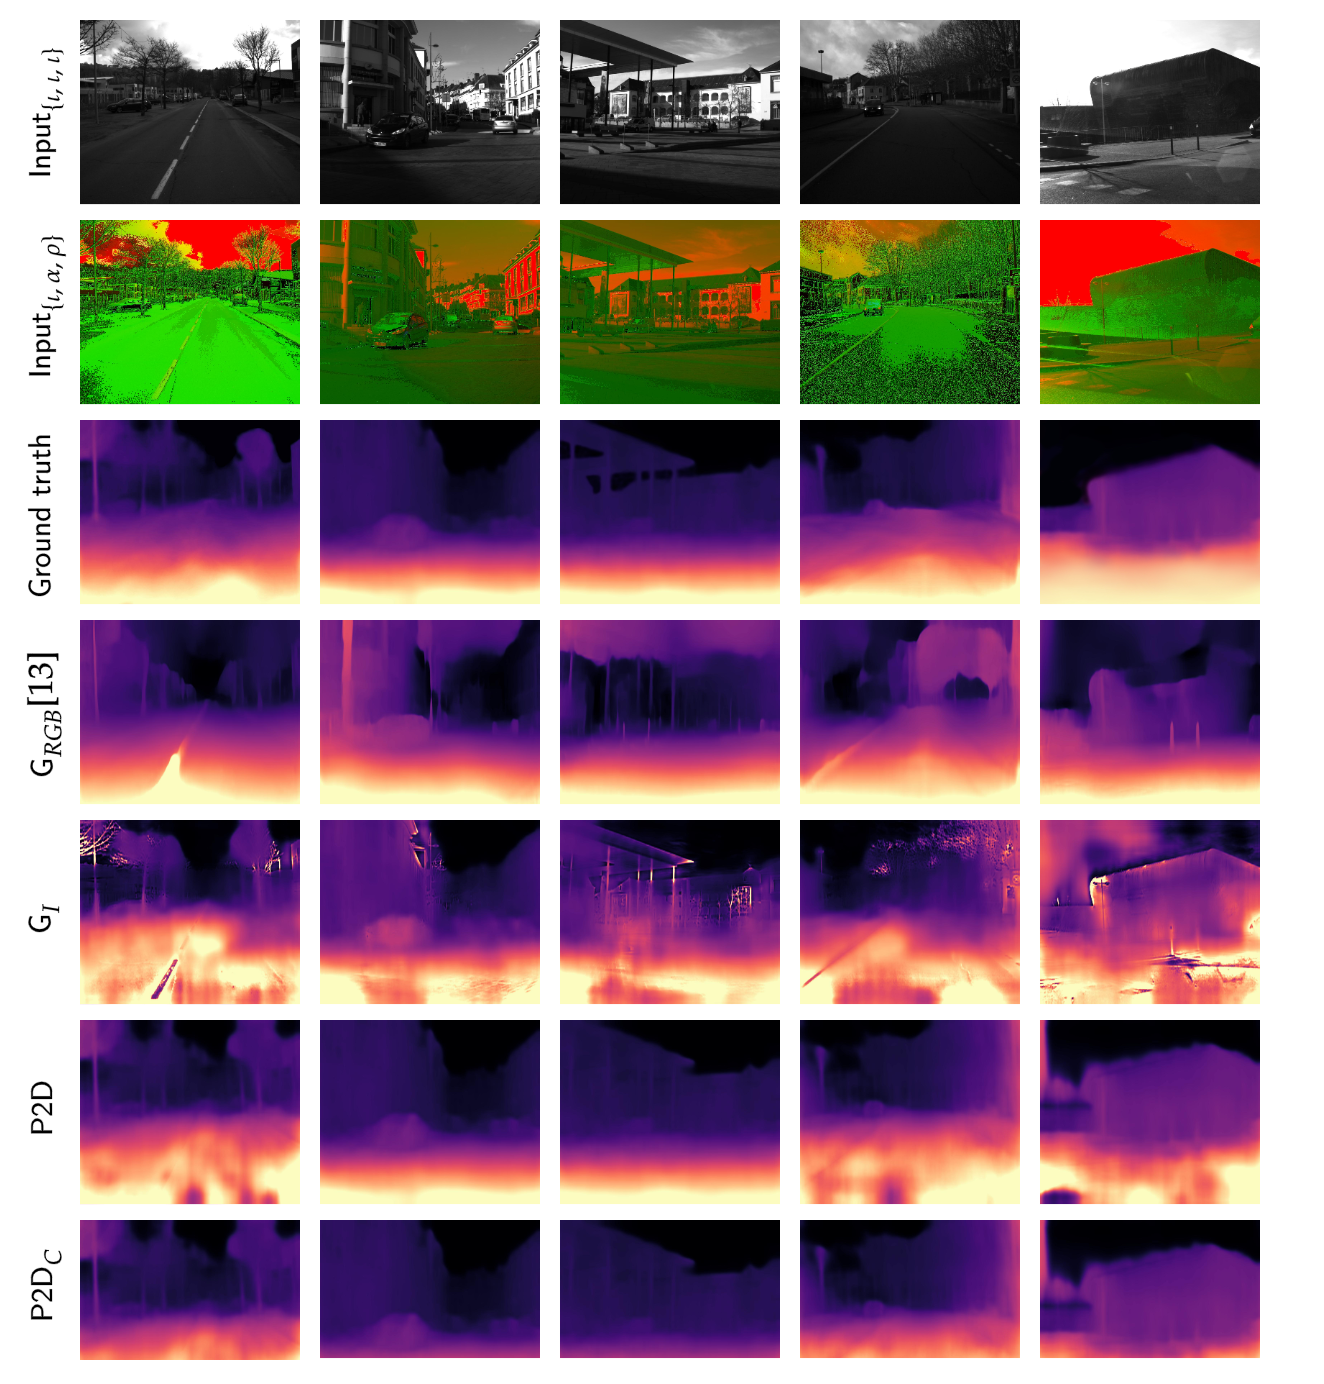
\includegraphics[keepaspectratio,width=.8\linewidth]{Figures/ECCV/results2}
	\caption[Illustration of results on five independent road scenes in mixed weather conditions.]{Illustration of results on five independent road scenes in mixed weather conditions. From top to bottom, the inputs to the two networks (scalar or polarimetric), the ground truth depth map, then the results of the three different networks: G$_{\textrm{RGB}}$ corresponds to the network presented in \cite{godard2019digging} without fine-tuning, and G$_{\textrm{I}}$ corresponds to the same network with fine-tuning. P2D corresponds to our method.
		The last row shows the crop version of the results from P2D to eliminate inconsistencies due to the modality and aberrations because of the camera position. Columns one and four correspond to acquisitions in light rainy weather, hence, the different road behaviour in polarimetric space. The other images are acquired under normal conditions.\vspace{.5cm}}
	\label{fig:res}
	
\end{figure*}





When the network is trained end-to-end with polarimetric intensity images, the global impact of polarization is reduced but brings many significant constraints. Despite an accurate estimation of some areas like planar surfaces on cars and long distance objects (see row G$_I$ in Figure~\ref{fig:res}), others areas are subject to some aberrations mainly on the reflective lines and polarized contours. This behaviour produces a direct impact on the network estimations.
Hence, the addition of polarization-specific terms is necessary to improve the estimation of polarized areas.

When employing all the polarimetric information ($\iota$, $\rho$ and $\alpha$) in our P2D network, we can observe a accurater estimation of specular areas as well as sufficient reconstruction of diffuse areas.\\
We can however see that the results at limited distances, as shown in the P2D row of Figure~\ref{fig:res}, are occasionally incorrect.
This is due to the fact polarimetric information varies according to the light and its reflection angle. Therefore, the position of the camera is primarily responsible for these erroneous estimates.
Indeed, as explained earlier in the Datasets section, the images of the evaluation subsets were acquired with different camera poses. Consequently, the information from the images differs from the training set case leading the network to fail in estimating depth values at close distances. 
To have an estimation in favorable conditions, the choice of cropping the lower quarter of the images for a second evaluation is proposed. Note, this lower part corresponds to closer distances. Both the estimates and the ground truth depth maps are cropped. 
These results are shown in the P2D$_\textrm{C}$ line of Figure~\ref{fig:res} as well as the \textit{Cropped} part of the Table~\ref{resmet}. We can observe better performances especially when comparing errors with the $\delta$ metric. The most considerable improvements are obtained when looking at both $\delta > 1.25$ and $\delta > 1.25^2$ showing a respective 16\% and 17\% improvement compared to the $G_{\textrm{RGB}}$ network.\\

Additionally, we perform an evaluation considering only the specular areas of the scenes. This is achieved using a rule-based naive system filtering polarization degrees higher than 0.4, hence keeping areas which are highly specular. 
The results shown in the last part of Table~\ref{resmet}, exhibit improved performances for all the evaluated networks since the assessed pixel space is reduced. However, the largest improvement is obtained with our P2D method. Specifically, our method achieves 92\% for $\delta > 1.25^2$ ratio, compared to 80\% obtained by the state-of-the-art method.
Consequently, we can see the polarimetric modality is beneficial for the reconstruction of urban scenes with many specular surfaces. 
Ultimately, to highlight the depth map reliability, sky reconstruction accuracy (eq.~\ref{reconSky}) has been computed in Table~\ref{Reconsky}.\\

\begin{center}
	\begin{table}[H]
		\centering
		\caption{Quantitative comparison of sky reconstruction accuracy.}
		\label{Reconsky}
		\begin{tabular}{c||ccc}
			\hline
			Network & $G_{RGB}$ & $G_{I}$ & P2D   \\ \hline \hline
			$R_s$      & 0.055     & 0.388   & \textbf{0.532} \\ \hline
		\end{tabular}
	\end{table}
\end{center}
This specific metric has been computed since many evaluation metrics neglect such aspect which, however, could be informative, especially if one uses such an algorithm for navigation. This ratio reveals P2D's ability to reconstruct slightly more than half of the sky correctly. It permits to demonstrate polarimetry to be favorable also for such estimation.


\section{Polarization and colorimetry fusion for accurate depth estimation: a theory}

Despite the innovative approach proposed in the previous section, it is notable that in the framework set, the problem is brought as an end-to-end learning problem.
That is, it is necessary to reconstruct an image, starting only from the polarimetric priors and without further information from other modalities.
This approach has demonstrated many qualities and highlights good performances. However, in some cases, this method tends to fail due to the lack of information or the annihilation of the perspective geometry term by the polarization.
In brief, the joint learning of the perspective geometry and the polarization geometry remain a complex task. It is sometimes possible to observe, as in Figure \ref{fig:polafail}, contradictions which lead the network to uncertain optimizations.

\begin{figure}[h]
	\centering
	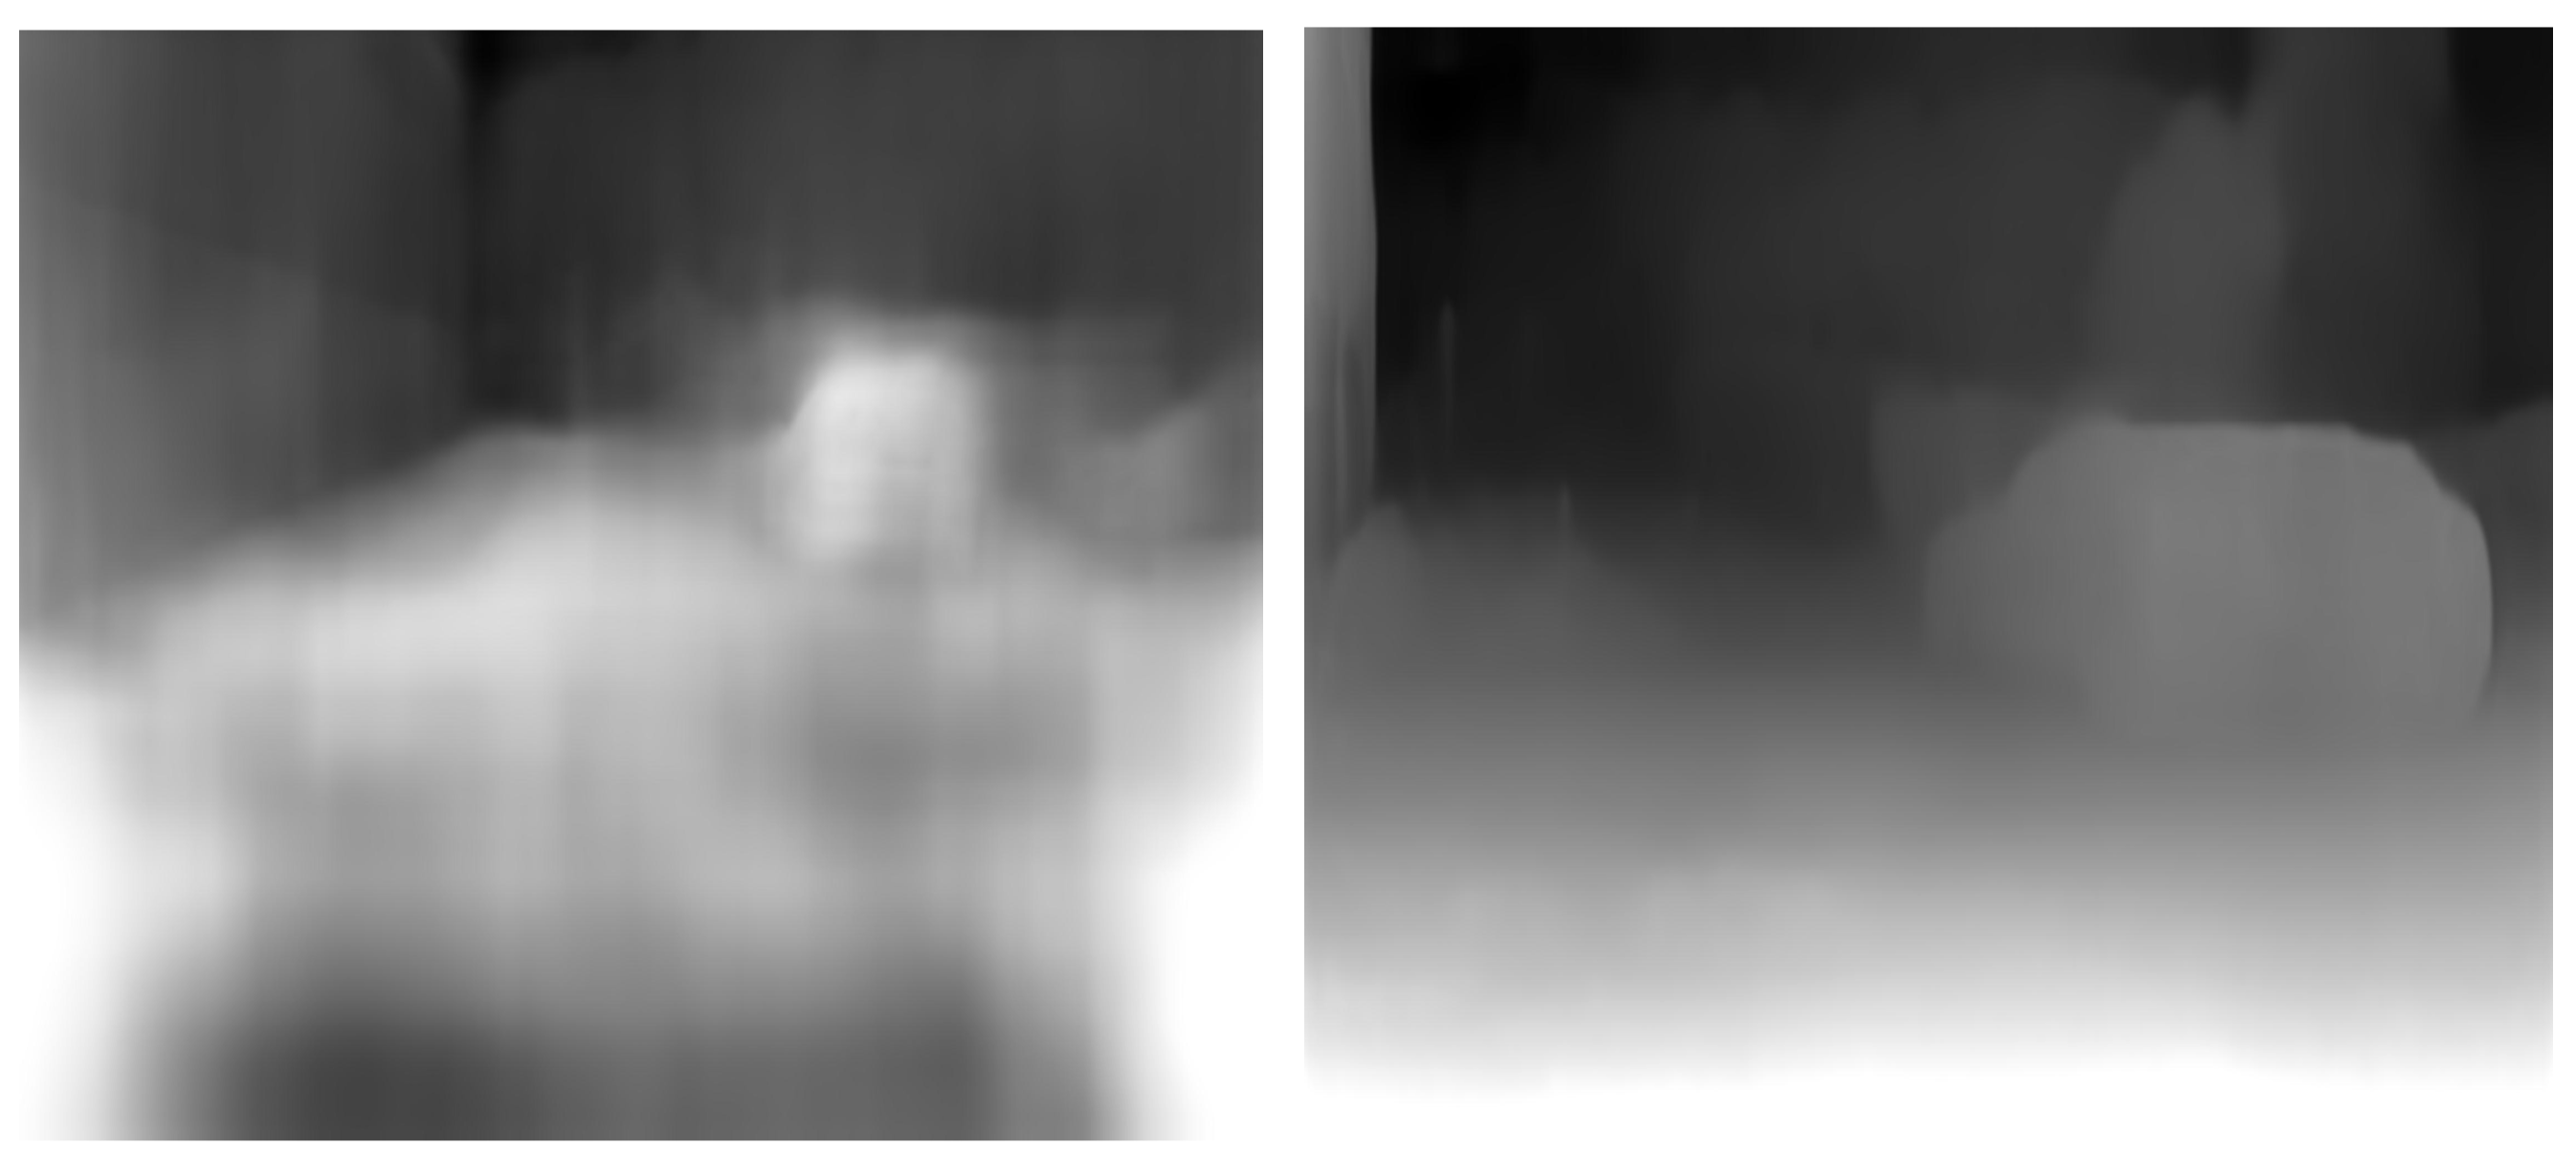
\includegraphics[width=0.8\linewidth]{Figures/Fusion/polafail}
	\caption[Case of estimation failure using P2D comparing to Monodepth v2.]{Case of estimation failure using P2D comparing to Monodepth v2. Left shows P2D estimation on polarimetric image. Right shows Monodepth v2 estimation on RGB similar image. Source images observe a car and both images were taken at the same time and under a colorimetry-favorable condition.}
	\label{fig:polafail}
\end{figure}


On the other hand, some colorimetry-based methods have been approved and are robust to many events. Although these approaches are directly related to the features present in the image, their learning with the help of massive databases allows strong abstraction capabilities.

The two principles contain contradictions but seem robust, hence, we propose to investigate the possibilities of merging the performances. As follows, the problem is no longer depth map estimation from polarization but a refinement of a map estimated from colorimetry using polarization.

\subsection{Estimating the appropriate fusion method}

There are multiple methods of merging. However, a small population of approaches allow multimodal image fusion, especially when one is physics-based.

We propose estimating the different possibilities of fusion of polarization and colorimetry. Thus, it will be possible to deduce which processes are applicable to theoretically obtain satisfactory results and especially to address the problem of depth map refinement.

\subsubsection{Early fusion}

Early fusion is a very common process since it is simple to implement. 
It basically consists of the image concatenation prior to the network. This technique requires perfectly aligned images and is frequently associated with 2.5D. Indeed, the RGB+D modality is extremely suitable since this information is complementary and can be aligned to the nearest pixel. 
Preliminary approaches like FuseNet \cite{hazirbas2016fusenet} or MVCNet \cite{ma2017multi} have proposed segmentation methods using early fusion. This kind of approach would be completely adaptable to a self-supervised depth learning problem by adapting the loss function.
A method close to our topic is RTFNet \cite{sun2019rtfnet} which proposes a semantic segmentation from a fusion of RGB and thermal image. This contribution highlights that it is possible to merge via this process images in two different spaces and especially colorimetry and a physics-based image.

It is nevertheless remarkable an overwhelming majority of the techniques are based on fusion applied to segmentation, although this is only an adaptation of the objective function to encounter a problem of depth estimation.


To assess whether this process is accessible to RGB polarimetric fusion, it is necessary to estimate the prerequisites for using such a method. The main idea is based on the concept of modality complementarity. Unfortunately, polarization and colorimetry share mutual information which would imply redundancies. It would indeed be possible to perform ablations to eliminate these redundancies or perform a thoughtful concatenation of the images. Thus, it would be possible to obtain a five-channel image composed of the three components of the RGB and the two complementary information of polarization, namely the angle and the degree of polarization. 


As shown in Figure \ref{fig:earlyf}, such an approach have been schematized.


\begin{figure}[h]
	\centering
	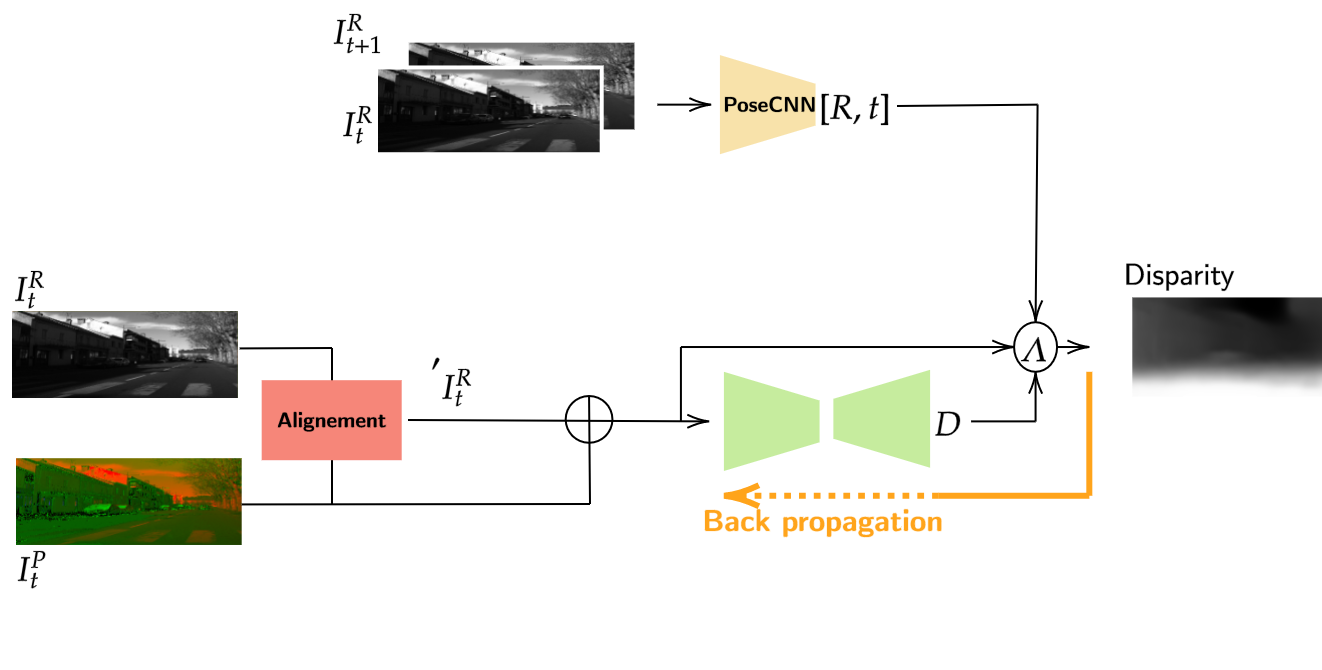
\includegraphics[width=0.8\linewidth]{Figures/Fusion/earlyf}
	\caption[Early Fusion architecture illustration.]{Early Fusion architecture illustration.}
	\label{fig:earlyf}
\end{figure}


As an intermediate conclusion, this kind of approach already requires a massive amount of aligned information. In addition, this specific technique almost necessarily requires an end-to-end depth estimation. The problem formulation is therefore not compatible with such an approach. The key concept is to take advantage of the robustness of RGB approaches and the specificity of P2D. As a consequence, early fusion does not address the problem since it is potentially subject to the same flaws as P2D. 
Another possibility relies not on a fusion before the network but in its core.

\subsubsection{Latent space fusion}

Latent space fusion consists in examining a strategy to combine several feature vectors from two different modalities.
The principle consists in having an encoder that extracts the main information from each channel and then accumulates it to mutualize the decoding process.


This concept can be based on statistical blocks, dense convolution layers or direct concatenation/addition to merge the information.
This is based on the assumption that information is combinable and therefore the decoder allows, despite different modalities, to extract mutual data.
However, most methods do not consider this point and assume that dimensionality remains the unique condition for fusion. Practice allows verifying this, but greedy algorithms such as deep learning are famous for their ability to reach an objective formulated by a function. This implies that whatever the type of data, valid or not, mergeable or not, the system will find an equilibrium point allowing to optimize the function. 

In our case, we consider the latent space fusion to tend towards the estimation of an accurate depth map. We must not neglect the fact that the two modalities have similar points and that the polarization brings a unique information allowing to optimize further. Some methods \cite{rashed2019motion,el2019rgb} have tried to merge these two data without deeply considering the impact of each modality and their influence for a semantic segmentation task.
A look-alike latent space fusion based architecture is schematized in Figure \ref{fig:latents}. This schematic is adapted to the problematic of depth estimation which explains the PoseCNN network.

\begin{figure}[h]
	\centering
	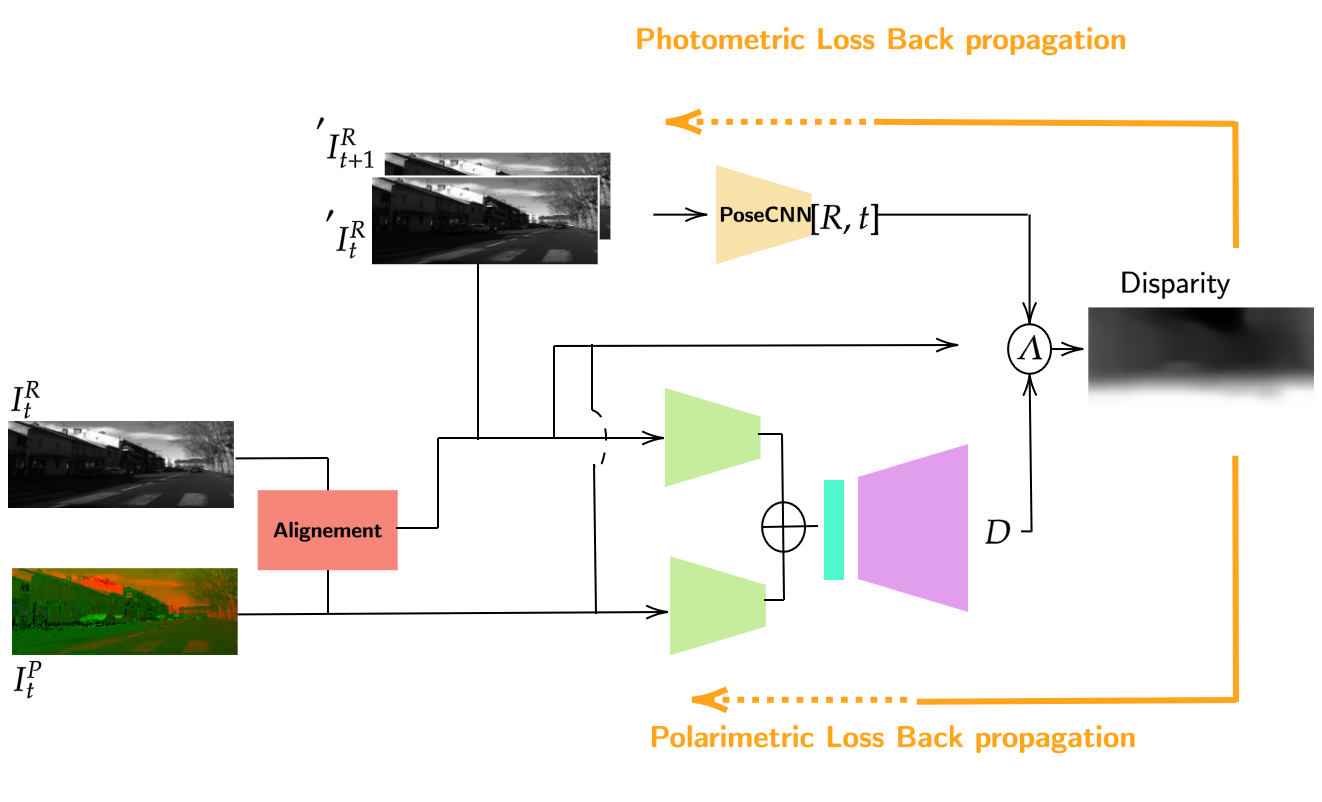
\includegraphics[width=0.8\linewidth]{Figures/Fusion/latents}
	\caption[Latent space Fusion architecture illustration.]{Latent space Fusion architecture illustration.}
	\label{fig:latents}
\end{figure}


For our approach, we consider it would be convenient to force the differentiability of non-mutual information.
One of the possibilities we propose to investigate theoretically is the use of sparse coding. These networks based on sparse coding formulate the problem as a reconstruction of the initial image with a tolerance. The weights of the network subsequently become a descriptive dictionary that allows, from the feature vector, to reconstruct the initial image.
This kind of network is traditionally trained by following a particular loss such that, given an input image $X$:

\begin{equation}
	\Lambda = \frac{1}{2} || X - Cy ||^2_2 + \lambda ||y||_1,
\end{equation}

with $C$ the the weight matrix, usually called dictionary in this field, and $\lambda > 0 $, a weighting tradeoff parameter controlling the sparsity of the feature vector $y$. Thus, this $\Lambda$ loss function aims to recover the initial image by penalizing the difference between the reconstruction and the initial image and ensure vector sparsity through L1 norm.

This kind of loss can allow for each modality to accurately describe the initial information. But in our case, the goal is to find a differentiable space allowing to discriminate and separate the polarimetric information from the shared information. Thus, this kind of context can be delimited as follows:

\begin{equation}
	y^p_p = y^p - y^r \quad with y^p = y^p_m + y^p_p,
\end{equation}

with $y^p$ and $y^r$ being respectively the feature vector from polarization and RGB image. Also, the indices $m$ and $p$ denotes for mutual and polarization.
Following this framework, it is possible to deduce two peculiar functions and more generally a joint loss allowing to reach this objective.

\begin{equation}
	\gamma = \Lambda_p + \Lambda_r + ||C_ry_r - ^{\{\iota\}}C_py_p ||^2_2
\end{equation}

with indiced $\Lambda$ a modality related sparse coding loss fuction such that \mbox{$\Lambda_p = \frac{1}{2} || X_p - C_py_p ||^2_2 + \lambda ||y_p||_1$}. In this formulation $^{\{\iota\}}C_py_p$ represents the polarization intensity $\iota$ related reconstruction. In such way, the polarization parameters are discrimated and the function ensure for an accurate reconstruction of both mutual information shared through RGB and polarimetry.

Then, with an ensured differentiable space between intensity and polarimetric parameters, it is possible to build an architecture allowing to take advantage of the supplementary information brought by the multi-modality without involving redundancy. Through this, the network can theoretically not be influenced as before by optimizing everything equally at once. The loss of photometric reconstruction as well as the estimation via PoseCNN can be operated exclusively on the mutual information while the polarimetry-related operations can be computed only with the polarimetric information.
This kind of approach additionally allows to make clear connections between the input and output of the pipeline by making the spaces separable and distinct.
Another considerable advantage of sparse coding is the economy of parameters. Through this kind of objective function, the general idea is to reconstruct a representative image at a more reasonable cost through the principle of sparsity.


In 2021, a promising approach \cite{wen2021sparse} integrating sparse coding has emerged. Indeed, it extracts colorimetric and polarimetric information acquired with a bimodal sensor through a sparse coding optimizer deduced dictionary.
This approach allows validating the hypothesis that these two information are separable. Moreover, the problem presented in the contribution is clearly more complex since the two pieces of information are, in the case of a bimodal sensor, physically merged. This confirms then the process described in this section can be exploited with two cameras with a prior image alignment or with one of the new cameras combining the two modalities into one.
Moreover, it is still complex and costly to generate joint models allowing the modelization of vectors that share mutual information while keeping their differentiability for polarimetric information. Furthermore, this end-to-end training can lead to other constraints that make the optimization function fall into local minima. It would be more convenient to take advantage of already estimated depth maps and then refine them. In this sense, it is then possible to evaluate the possibilities of using a late fusion architecture.


\subsubsection{Late fusion}

Another possibility is based on a posteriori fusion from the networks. It consists in the encoding of two independent images towards a common space in which a fusion will be possible. Similar to latent space fusion, where the common space is examined during the intermediate step before decoding, here the common space is deduced at the end of the network for the two separate images.
Next, it is a matter of finding a strategy to assemble these two transposed images to reach a final goal.

The general principle is based on two independent networks and then a final simple or multilayer network that will learn a fusion strategy.

This approach is totally suitable to the formulated problem, but the objective is shifted to the estimation of an objective function allowing the optimal fusion from the common space. In a first step, the intermediate objective can be set, namely to convert the source images.
In our case of depth map refinement, the representation would then be a depth map specific to each modality. Thus, it would be possible to formulate two cost functions that would infuse the characteristics of each modality to obtain two accurate depth maps.

As shown in Figure \ref{fig:late1}, a preliminary per-modality depth estimation can be performed.

\begin{figure}[h]
	\centering
	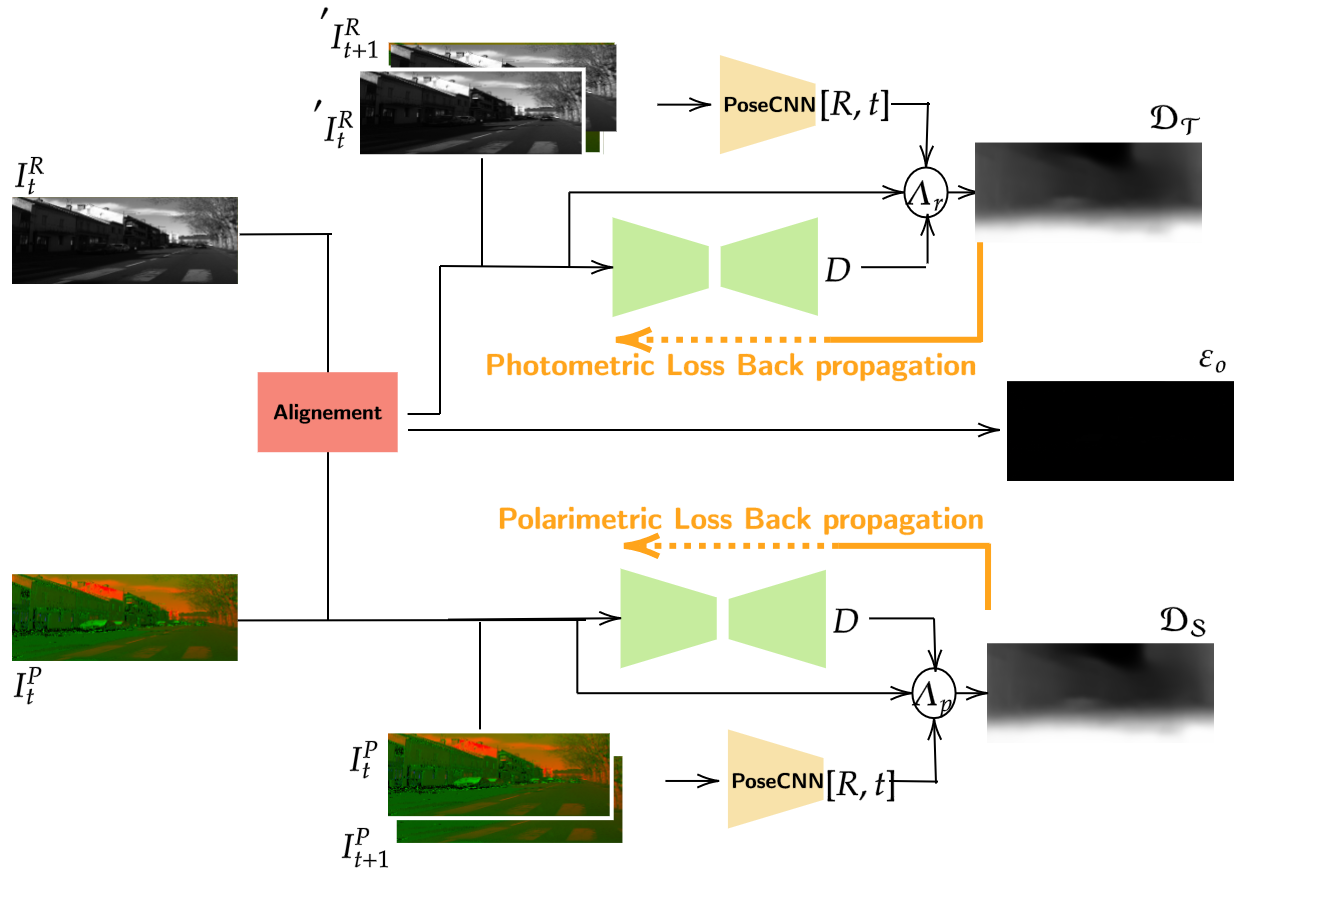
\includegraphics[width=0.8\linewidth]{Figures/Fusion/late1}
	\caption[Late Fusion architecture illustration. Prior Estimations.]{Late Fusion architecture illustration. Prior Estimations.}
	\label{fig:late1}
\end{figure}


A first pipeline can consider the colorimetric modality by adopting the strategy of Godard et al. with its formulation of photometric error, smoothing and taking into account the occlusion and parallax parameters.
A second pipeline addressing the polarization could only regularize the normals to match the polarization angle. This strategy would allow obtaining sparse images but loaded with information where the polarization can be impactful. Discrimination with respect to the degree of polarization is then valid to consider only specular surfaces and to verify the equations relating normals and $\alpha$. This approach would be a P2D relieved of the constraints of photometry-based perspective geometry.

At the end of these two pipelines, two depth maps would be obtained, one built using the perspective geometry formulation and the other verifying the validity with respect to polarimetry.
Finally, these two maps could be aggregated using a fusion network based on raw uncertainty measurements. A strategy framework is proposed in Figure \ref{fig:late2}.

\begin{figure}[h]
	\centering
	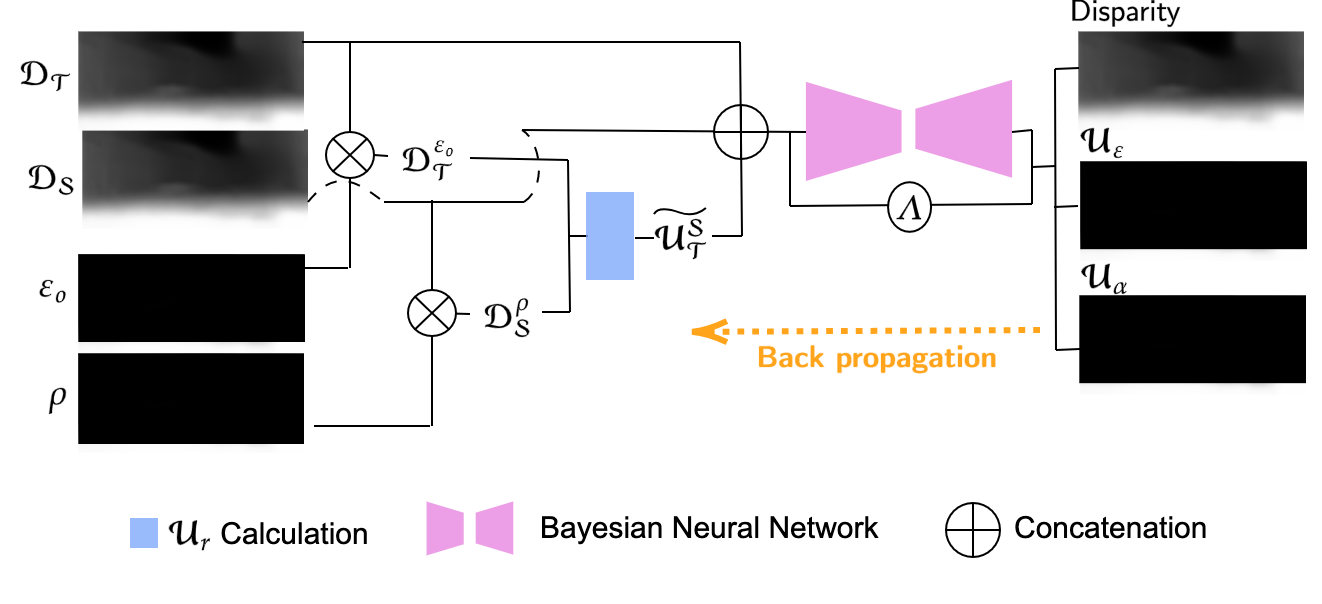
\includegraphics[width=0.8\linewidth]{Figures/Fusion/late2}
	\caption[Late Fusion architecture illustration. Late refinement.]{Late Fusion architecture illustration. Late refinement.}
	\label{fig:late2}
\end{figure}

This uncertainty measure must integrate the errors inherent to the modalities or the cross modality alignment.
We rectify the depth map according to the different errors that are available such as $\varepsilon_o$ the alignment error and $\rho$ the degree of polarization. We justify this rectification by contextualizing the disparate impact of those parameters. While RGB image has been rectified, polarization cannot be affected by any transformation. Ultimately, the alignment error is impacted and due to the polarimetric modality. As for propagating the degree of polarization on the radiometry-based estimation, this is necessarily due to the lack of modality knowledge. Colorimetry based information do not observe any specularity awareness except by saturation. In highly specular area, it is a benefit to acknowledge such high impact data. In addition, most colorimetry-based monocular depth estimation approach are known to highly perform in textured/features regions and as contrary, to fail in different other cases (the saturation being one of those cases ). In accordance, we scale inferred estimation by the inverse of $\rho$ to manage those specific uncertainty as follows:
\begin{equation}
\begin{cases}  
\mathcal{D}_{\mathcal{T}}^{\varepsilon_o} =  \mathcal{D}_{\mathcal{T}} \times \rho\\[8pt] 

\mathcal{D}_{\mathcal{S}}^{\rho} =  \mathcal{D}_{\mathcal{S}} \times \varepsilon_o

\end{cases}.
\end{equation}

$\mathcal{D}_{\mathcal{T}}$ and $\mathcal{D}_{\mathcal{S}}$ are respectively the dispartities deduces from colorimetry and polarimetry. By substracting both the deduced depth maps, a new cross-modality estimation uncertainty can be computed such that:

\begin{equation}
	\widetilde{\mathcal{U}_{\mathcal{T}}^{\mathcal{S}}} = |\mathcal{D}_{\mathcal{S}}^{\rho} - \mathcal{D}_{\mathcal{T}}^{\varepsilon_o} |.
\end{equation}


Another ultimate procedure to estimating uncertainty $\mathcal{U}$, although always relative since it is a student-teacher approach, is the method proposed by Poggi et al. \cite{poggi2020uncertainty}:

\begin{equation}
\widetilde{\mathcal{U}_{\mathcal{T}}^{\mathcal{S}}} = \frac{|\mu(\mathcal{D}_\mathcal{S}) - \mathcal{D}_\mathcal{T}|}{\sigma(\mathcal{D}_\mathcal{S})} + \log (\sigma(\mathcal{D}_\mathcal{S}))
\end{equation}

The two previous methodologies have the advantage of requiring no tedious additional processing. However, as specified above, there is the notion of relativity which tends to imply the relative optimal is not the absolute optimal.

Now that we have three characteristic images, we need to consider a strategy to merge this information to refine a depth map.
We propose a concept based on a Bayesian Neural Network (BNN) \cite{denker1990transforming,mackay1992practical}. Indeed, this kind of architecture allows modeling \emph{epistemic} and \emph{aleatoric} uncertainty \cite{der2009aleatory}. As expressed in \cite{kendall2015bayesian,kendall2016modelling} and \cite{kendall2017uncertainties}, these two uncertainties allow to estimate respectively the robustness of the network and the impact of the data (mainly if it is subject to noise).
Our singular goal is to refine a depth map and epistemic uncertainty modeling seems an excellent candidate to optimize in this direction. 
The overall idea would be to minimize the cross-modality uncertainty jointly with the epistemic uncertainty.
This approach is almost necessary because there is no conspicuous domain where one can regularize two disparity measures. Such a method allows to have a differentiation and force the use of information coming from both modalities by the availability of $\widetilde{\mathcal{U}_{\mathcal{T}}^{\mathcal{S}}}$.
Finally, as shown in Figure, it is possible to schematize this unsupervised architecture taking advantage of relative uncertainties but also of a global uncertainty modeled by the BNN. 

In conclusion, this complex architecture would theoretically allow refining a depth map by taking advantage of both modality information and a complex uncertainty modelization through a BNN. On the other hand, this kind of setup requires a massive amount of data but especially a hardware architecture supporting an immense load of calculations. This constraint is directly attributed to the use of Bayesian neural network, simulating a large number of weights through Gaussian distributions.
To reduce this charge and to make it feasible in the short term, a cascade modeling that would benefit from prior estimates could be advantageous.

\subsubsection{Cascaded approach}\label{casc}

The cascade approach is radically different from the previous ones since, in addition to not requiring end-to-end training of each pipeline, it is expected to take advantage of pre-learned components without altering the preliminarily observed results.

First, one takes the pre-trained Monodepth v2 network. The results inferred from an RGB image are almost optimal under favorable conditions but tend to deteriorate in the presence of specularity. 
We propose taking advantage of these estimates and to refine them in a second step using another network infused with polarization parameters.
As shown in Figure, the cascade architecture is articulated in a single pipeline with two independent non-communicating estimation cores.



The main idea is to concatenate the pre-estimated depth map with the polarization parameters $\iota$ and $\rho$. It is then possible to deduce a loss function which, using each of these channels, will in self-supervised manner; train the model to the unique locations where the RGB estimation fails.
This objective function can be expressed as a function of the normals since the polarization angle allows to regularize them.

One can estimate a surface normal map from a depth map through oriented derivatives:

\begin{equation}\label{normes}
	\Delta \mathcal{D} = 
	\begin{bmatrix}
	g_x \\ g_y
	\end{bmatrix} =
	\begin{bmatrix}
	\frac{\delta \mathcal{D}}{\delta x} \\ 	\frac{\delta \mathcal{D}}{\delta y}
	\end{bmatrix}.
\end{equation}
\begin{equation}\label{normes2}
	\vec{n} = \begin{bmatrix}
	-g_x\\-g_y\\1
	\end{bmatrix}.
\end{equation}

As shown in Figure \ref{fig:normalsfromcube}, from a depth map, one can compute the according normals field.

\begin{figure}[h]
	\centering
	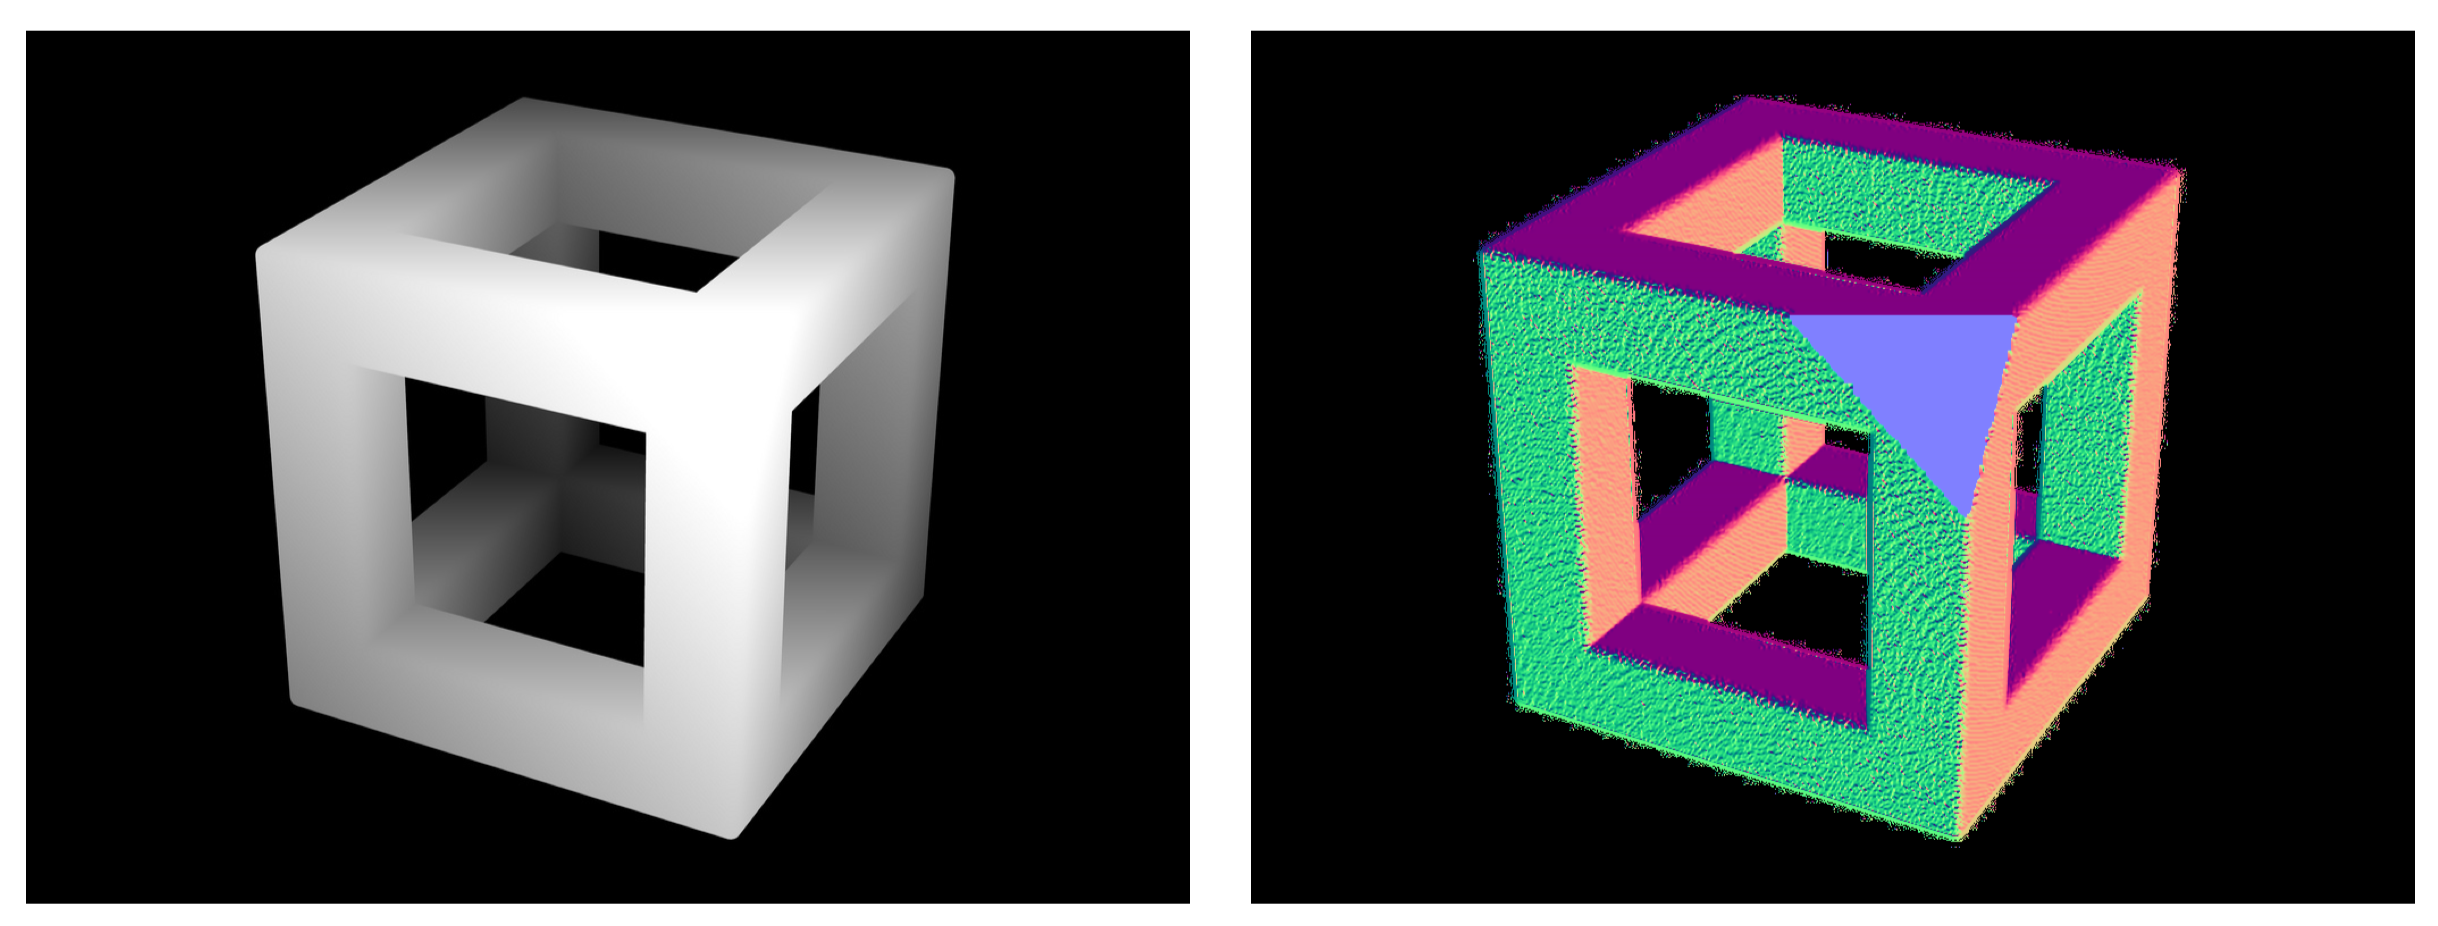
\includegraphics[width=0.8\linewidth]{Figures/Fusion/normalsfromcube}
	\caption[Illustration of depth to normals through oriented derivatives.]{Illustration of depth to normals through oriented derivatives.}
	\label{fig:normalsfromcube}
\end{figure}

From this normals field , it is possible to calculate the angle in relation to the reference axis which will allow a simplified comparison with $\alpha$:

\begin{equation}\label{ntoa}
	\Theta = tan^{-a}\Big( \frac{g_y}{g_x} \Big).
\end{equation}

Knowing the angle of polarization with normal orientation uncertainty and inspired from \cite{cui2017polarimetric}:

\begin{equation}
	A (\alpha, \Theta) = min(|\alpha - \Theta - \pi| , |\alpha - \Theta| , |\alpha  - \Theta + \pi|),
\end{equation}

with $min$ operation allowing for accountance of polarimetry-related angle uncertainty with respect to the surface.
Then, taking into account only specular surfaces and their related orientation uncertainty:

\begin{equation}\label{regu}
	L_{pol} = \rho A(\alpha + \frac{\pi}{2} , \Theta).
\end{equation}

Consequently, $L_{pol}$ represents a self-supervision-compatible error term considering both the polarimetric information and the initial estimate from the colorimetry. $\rho$ is adequately used to consider only the pixels where specularity is observed and the relation $\alpha$ to $\vec{n}$ is verified.


This solution, although the others are potentially viable, seems to be the most appropriate and above all can allow for theory-testing prior experiments without the need for a large-scale dataset.

\subsection{Prior experiments}

To verify the cascade network theory, we propose a first evaluation of an image processing based method. This approach is in all respects similar to the principle expressed in Section \ref{casc}.

Starting with a depth map estimate from Godard et al. \cite{godard2019digging}, it is possible to deduce a normal map with equations \ref{normes} and \ref{normes2}.

\begin{figure}[h]
	\centering
	\begin{subfigure}[b]{.8\linewidth}  
		\centering
		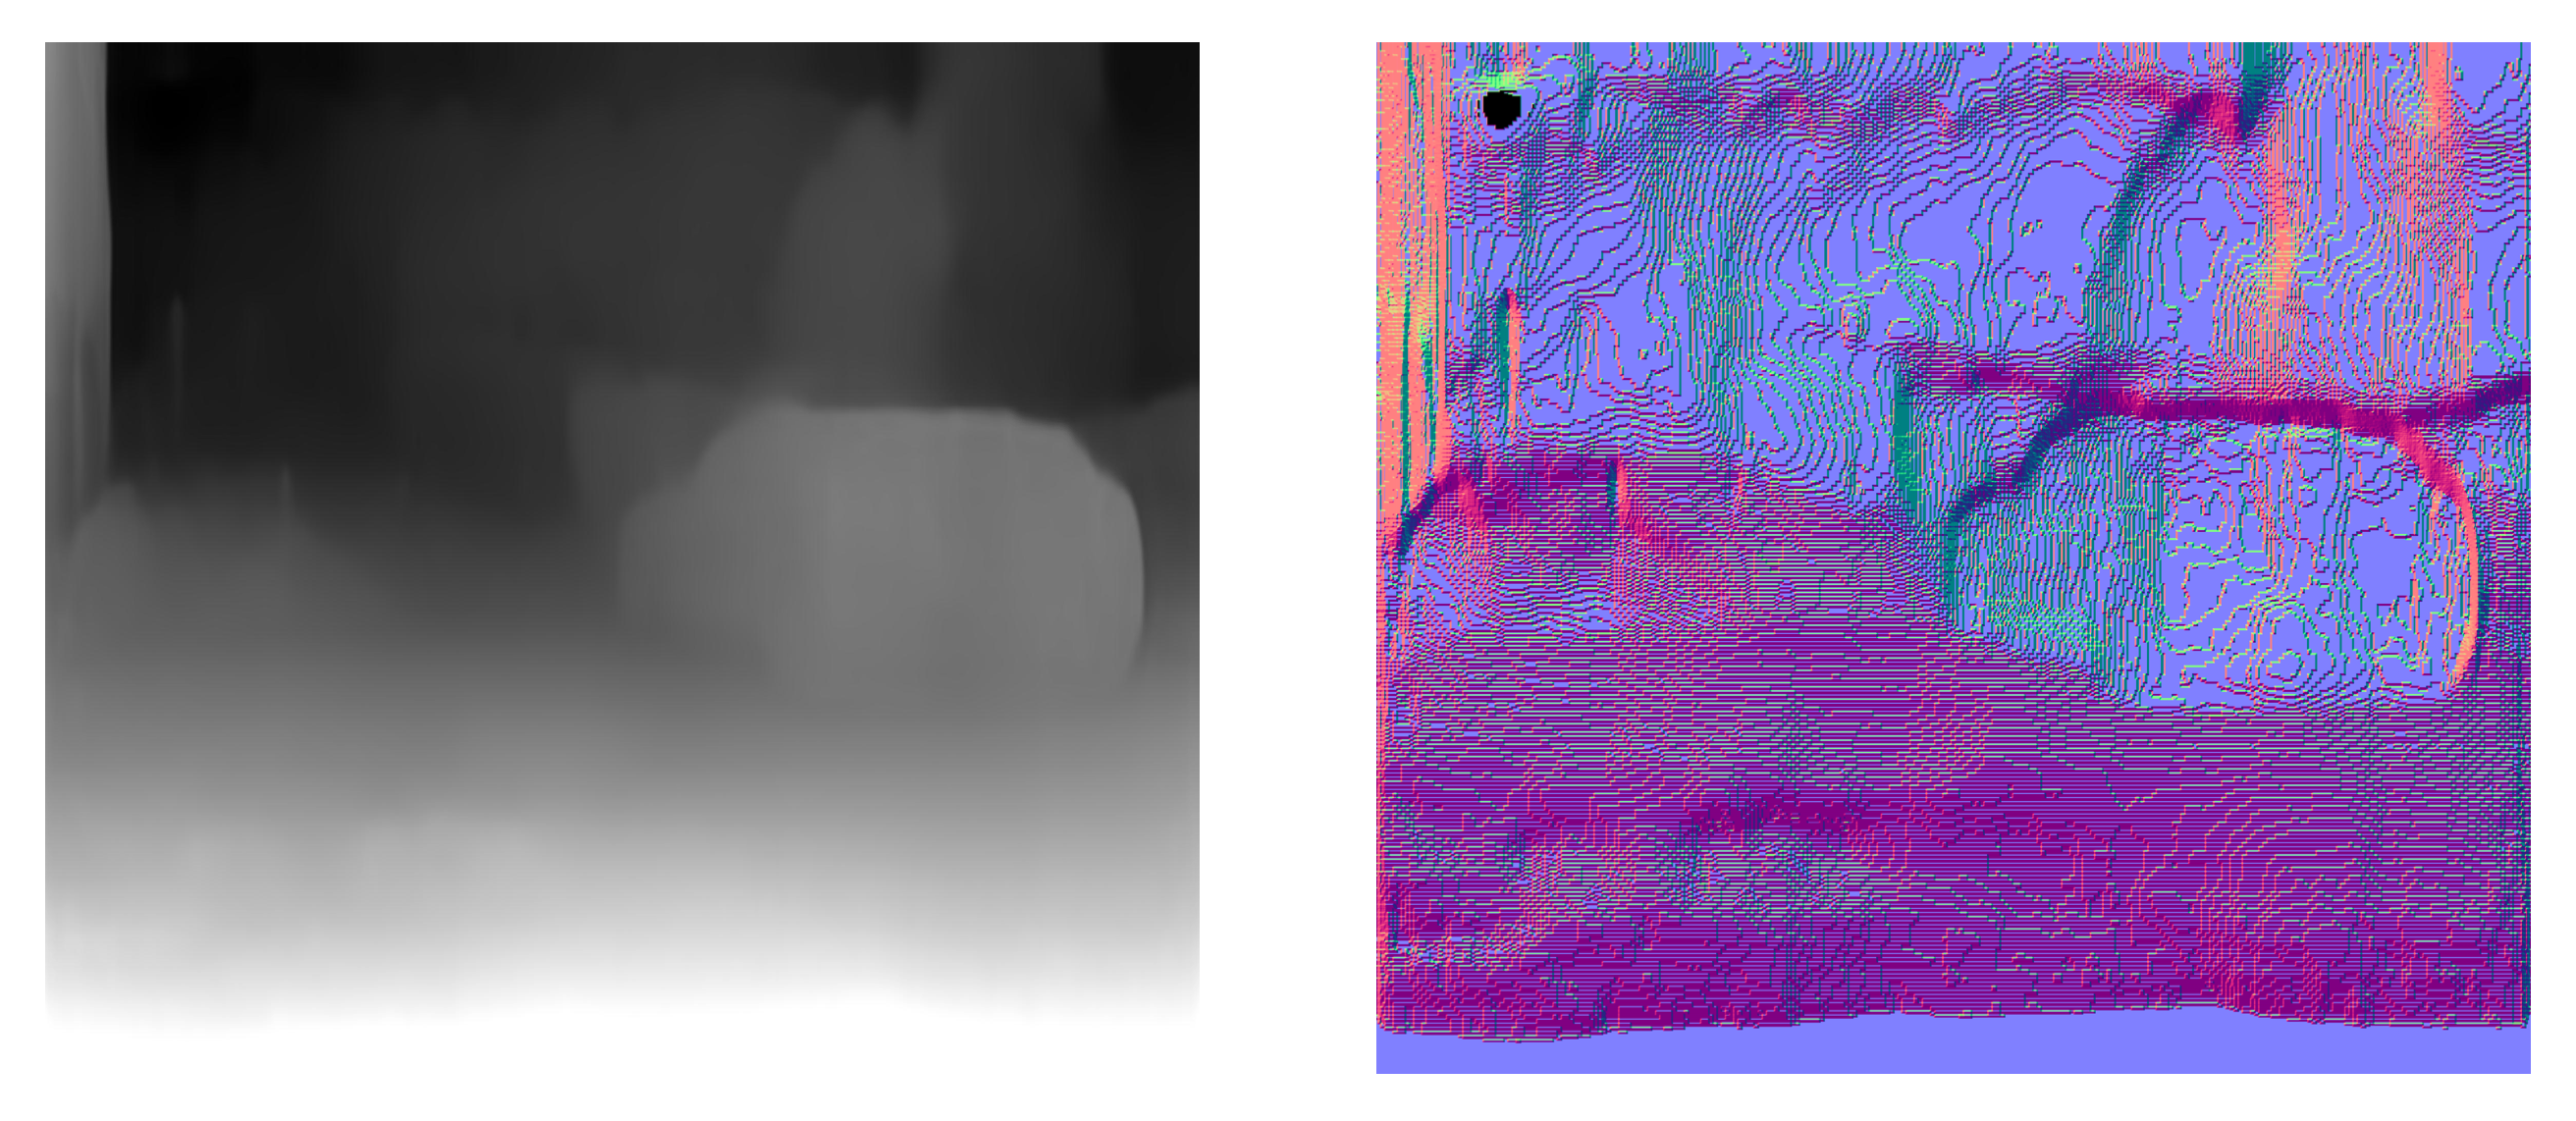
\includegraphics[width=\linewidth]{Figures/Fusion/normals}
	\end{subfigure}

	\begin{subfigure}[b]{.8\linewidth}  
		\centering
		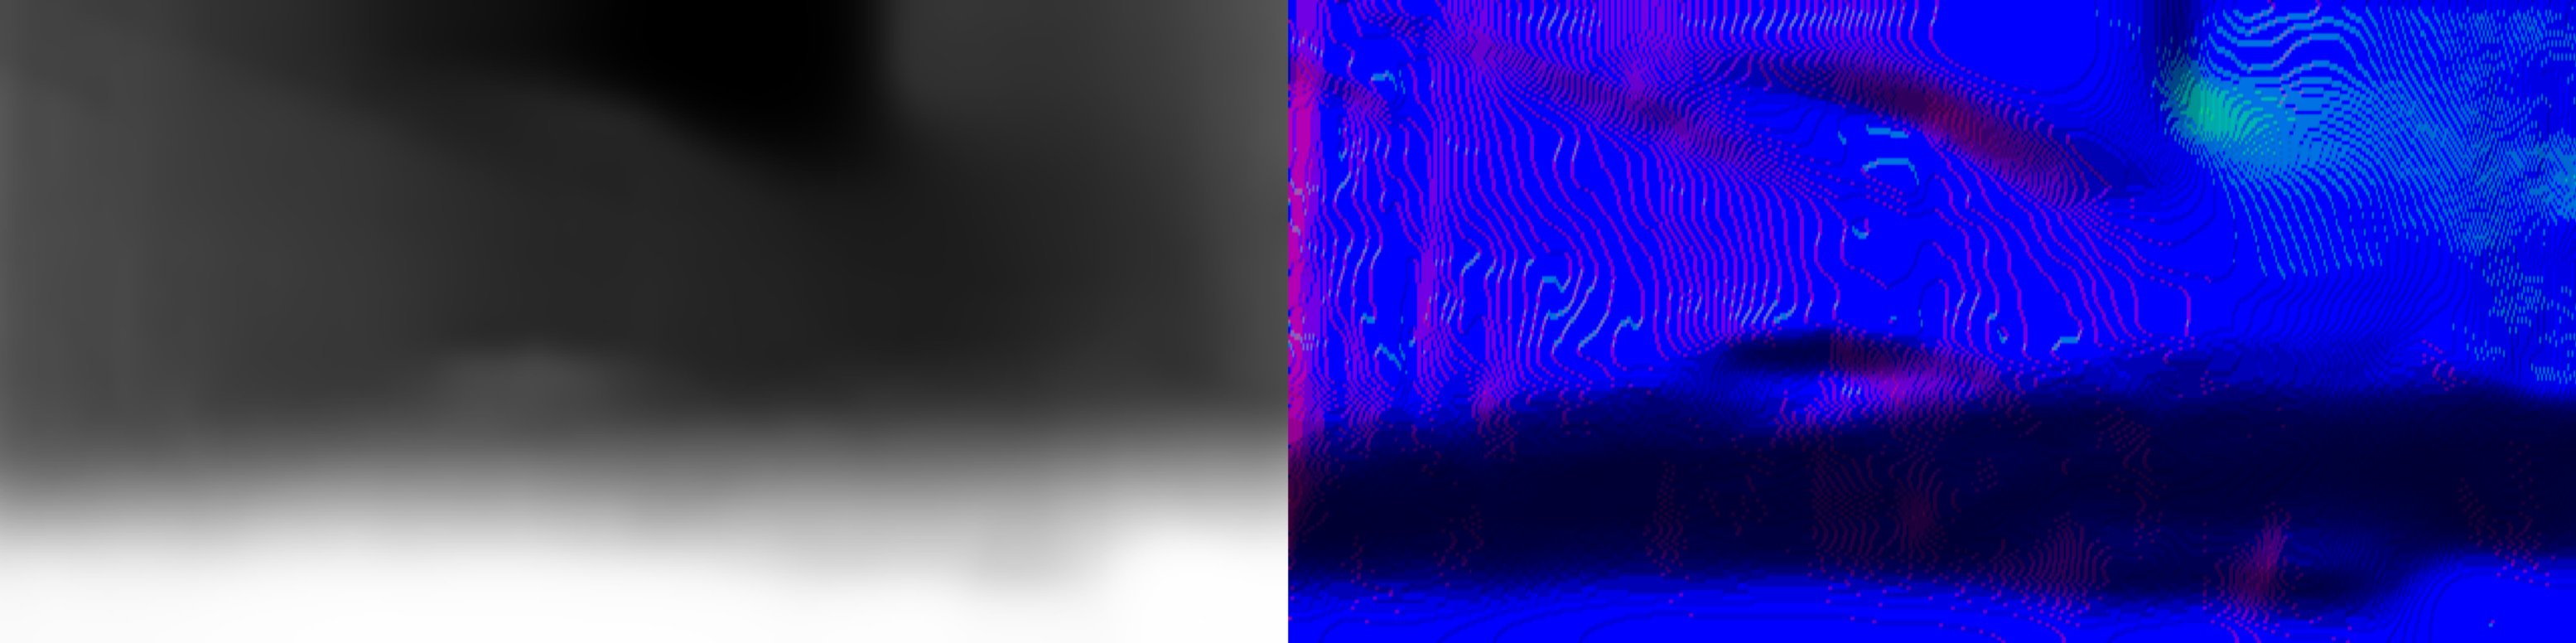
\includegraphics[width=\linewidth]{Figures/Fusion/godnorm}
	\end{subfigure}
	\caption[Normals estimation from Monodepth v2 estimate on two different scenes.]{Normals estimation from Monodepth v2 estimate on two different scenes. Left column shows the depth image and right column the correspond computed normals.}
	\label{fig:godnorm}
\end{figure}

As shown in Figure \ref{fig:godnorm}, the resulting orientations are discussable. Espacially in top row, normal vectors does not highlight properly the surfaces and tends to produce fictive shapes. \\
Assuming the normals field optimal (considering bottom row), one can compute the correspond angles following equation \ref{ntoa}. A resulting grayscale image shown in Figure \ref{fig:tan} can be displayed where $\Theta\in\left[0,\pi\right]$.

\begin{figure}[h]
	\centering
	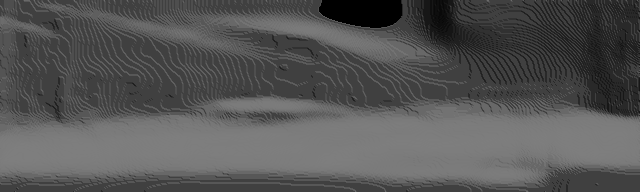
\includegraphics[width=0.8\linewidth]{Figures/Fusion/tan}
	\caption[Angles computed from normals.]{Angles computed from normals compted following equation \ref{ntoa}.}
	\label{fig:tan}
\end{figure}

In addition, the aligned angle of polarization $\alpha$ used for regularizing the previous angle map is shown in Figure \ref{fig:angleofp}.

\begin{figure}[h]
	\centering
	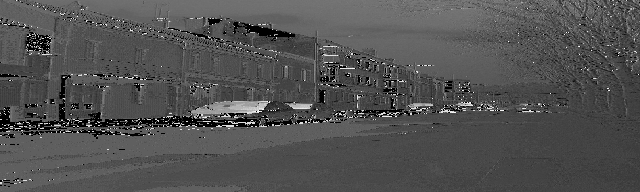
\includegraphics[width=0.8\linewidth]{Figures/Fusion/angleofp}
	\caption{Aligned angle of polarization.}
	\label{fig:angleofp}
\end{figure}

Subsequently employing the two previous informative images, one can estimate the error through equation \ref{regu}. $\rho$ is subsequently enforcing the computation on specular surfaces and reducing the impact of polarization characteristics to only the desired area. As shown in Figure \ref{fig:resim}, only few pixels are erronously estimated by the state-of-the-art colorimetry-based method. Consequently, this peculiar loss only focuses on these specific portions of the image that are specularity impacted.

\begin{figure}[h]
	\centering
	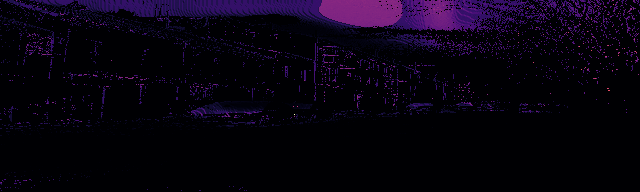
\includegraphics[width=0.8\linewidth]{Figures/Fusion/resim}
	\caption[Resulting error image from normal angles comparison.]{Resulting error image from normal angles comparison. The error is displayed following a colormap encouraging contrast. Thus, the brighter the higher.}
	\label{fig:resim}
\end{figure}

To obtain a back propagation compatible error, the only missing element lie into either averaging or summing the image. The optimal results being full black image.

Thanks to the limited number of impacted pixels due to $\rho$ filtering, the summation seems to represent the most ideal candidate avoiding vanishing gradient issues. 

Ultimately, this technique while considering colorimetry only involve the training of a polarization related network. This strategy is subsequently valid since the announced problem statement requires such a behaviour. 

\subsection{Discussion and conclusion}

While P2D allowed a first step towards depth estimation by polarization alone, it observed aberrations in particular cases. 
In another domain, approaches requiring RGB information include specific sensitivities due to the modality used. Thus, specularity remains a notable weakness in this kind of algorithm.

To establish a generic polarimetric based method, some fusion architectures have been investigated. Starting with an estimation of the theoretical possibilities and needs, we have proposed a plausible panel of architectures that can combine the two modalities. This study has allowed to highlight the inability of some methodologies to face multimodality problems reliably. Since we had delimited the problem, no longer as an end-to-end estimation but as a refinement, many complex architecture were conceivable. This complexity and the prerequisites of these methods (namely latent space fusion and late fusion) indexed our study towards a cascade architecture.
To prove the concept and since the process allowed it, we proposed to consider a no-learning experiment in real-like conditions. This proof of concept highlighted the possibility of operating such an algorithm.

Nevertheless, other methods requiring much higher computational power is still plausible and remain candidates to perform an accurate depth estimation/refinement task from polarization.

\section{Summary}

This chapter addresses the problem of depth estimation from polarization. Such polarization-based and unique methods are undoubtedly at a preliminary stage. However, the multiple approaches have highlighted that polarization can allow, through different information, to infer depth maps in a whole new way. 
P2D is, to our knowledge, the first-of-its-kind method proposed to infer a depth map from a polarimetric monocular and a DCNN. The results, although very promising, has displayed some weaknesses.
In response to these erroneous estimates, we proposed examining the possibilities to go farther in the field by exploiting preliminary achievements in RGB. This study allowed us to evaluate the possibilities of fusion and eliminate the candidates which were unsuitable for the task. Ultimately, we proposed, only in image processing for the moment, to determine if a fusion approach was viable.
We conclude that apart from Early Fusion, there is a vast possibility to improve the results of P2D and especially to make the approach more generic. However, the data barriers remain the principal obstacle, especially in the area of exploitation of specific unconventional data. We are confident that over time, as more polarimetric data become available, the greedy algorithms can be viably used to finally exploit these data.
Due to this lack of data, some experiments were conducted without learning. Despite this, these experiments have validated this proof of concept and could be exploited as soon as a dataset emerges in the scientific community.

In conclusion, we have proven polarization remain a discriminative modality that, when used judiciously, could improve the performance of algorithms for geometric understanding of urban scenes.


